\documentclass[11pt,halfline,a4paper]{ouparticle}

% \usepackage[T1]{fontenc}

\usepackage{mathptmx}
\usepackage{times}
\usepackage[flushleft]{threeparttable}
\usepackage{graphicx}
\setlength\parindent{12pt} 

\usepackage{tabularx}% http://ctan.org/pkg/tabularx
\newcolumntype{Y}{>{\raggedleft\arraybackslash}X}% raggedleft column X

% \usepackage{subcaption}
\usepackage{caption}
\usepackage{booktabs}
\usepackage{natbib}
\usepackage{rotating} % Load the rotating package
\usepackage[hidelinks]{hyperref}
\hypersetup{
  colorlinks   = true, %Colours links instead of ugly boxes
  urlcolor     = blue, %Colour for external hyperlinks
  linkcolor    = blue, %Colour of internal links
  citecolor   =  red %Colour of citations
}
\usepackage{xcolor}

\begin{document}

\title{Characteristic-based factors and exposure to macroeconomic risks
% \break {Second Line Title\thanks{We thank...}}
}

\author{%
\name{Xuanheng Huang}
\address{Bocconi University, Department of Accounting,\\
Milan, 20136, Italy}
\email{xuanheng.huang@unibocconi.it}
\and
\name{Peter Pope}
\address{Bocconi University, Department of Accounting,\\
Milan, 20136, Italy}
\email{peter.pope@unibocconi.it}}

\abstract{This paper investigates the ability of characteristic-based factor models to capture and account for macroeconomic risk. We study how benchmark factor models \citep[e.g.,][]{fama2015five,carhart1997persistence,hou2021augmented} relate to a factor model based on macroeconomic fundamentals. In particular, in the macroeconomic model, we consider five factors: changes in growth expectation, unexpected inflation, changes in the aggregate survival probability, changes in the average level and the slope of the term structure, and changes in the currency exchange rate. The findings in this paper could potentially explain the reasons behind the varying performance of characteristic-based factor models over time, specifically in the context of regime changes. }

\date{\today}

\keywords{Asset pricing; Fama and French model; Macroeconomic factors; Momentum; q-factor model; and Regime switching}

\maketitle

\newpage

\section{Introduction}

In recent years, researchers have proposed new factor models \citep[e.g.,][]{fama2018choosing,fama2015five,hou2021augmented}. However, the performance of characteristic-based factors has shown significant variation over time. Following the financial crises of 2007-2009, the returns of the factors from the Fama and French (FF) model have remained stagnant, despite the increasing equity market returns (see Figure \ref{fig:cumret_ff}). This puzzling phenomenon has motivated some papers to understand the underlying causes. For instance, \cite{herskovic2023micro} attribute the divergent performance between the equity market premium and the size and value premium to fluctuations in micro and macro uncertainty. In our study, we take a different approach. Previous research has explored the relationship between the FF factors and the risk derived from macroeconomic fundamentals \citep[e.g.,][]{aretz2010macroeconomic,hahn2006yield,petkova2006fama,vassalou2004default,vassalou2003news,liew2000can}. By examining this relationship and analyzing its changes over time, we aim to shed light on the time-varying performance of the FF model. Specifically, our objective is to ascertain whether the observed change in performance is derived from a regime shift, indicating an altered relationship between characteristic factors and macroeconomic risks. 


% In the context of APT \citep{ROSS1976341}, macroeconomic fundamentals matter because they capture common variations in equity returns or, the context of the ICAPM \citep{merton1973intertemporal}, macroeconomic risk matter because they capture the state of the word. The macroeconomic factor model directly tries to capture the macroeconomic fundamentals. 


% By studying the relationship in different subsamples we are able to document the changes in relationship between the two models. One reason for the varying performance may due to the fact that characteristic factor capture no differently macroeconomic risk.


Our study focuses on examining the benchmark FF model from the perspective of a macroeconomic factor model. To accomplish this, we use the comprehensive macroeconomic factor (MF) model proposed by \cite{aretz2010macroeconomic}. First, I investigate the univariate correlations between the factors derived from both models. Furthermore, we explore how characteristics relate to macroeconomic risk by estimating the exposure of one-way sorted portfolios, based on characteristics, to each of the macroeconomic factors. 

By exploring the relationship in different subsamples, we can identify and document any changes in the relationship between the FF model and the macroeconomic factor model. We seek to understand whether the varying performance of the characteristic factors can be attributed to a regime shift that occurred after the financial crisis.

% I find this and this.

% I plan to do this and this.

The rest of the paper is organized as follows. In Section \ref{literature}, we review the literature. In Section \ref{RD}, we explain the empirical methodology and describe the data. In Section \ref{results}, we show and comment on the results. In Section \ref{plan}, we outline the plan for future drafts.

\section{Prior literature}
\label{literature}

Working in progress...

% Previous work that study the association between fama french  and macroeconomic fundamentals

% \cite{liew2000can}: GDP growth on market, book-to-market, size and momentum. Can book-to-market, size and momentum be
% risk factors that predict economic growth?

% \cite{hahn2006yield}: "small stock portfolios have higher loadings on $\Delta def$ than large stock portfolios, while high book-to-market portfolios have higher loadings on $\Delta term$ than low book-to-market portfolios". "small firms tend to be young, poorly collateralized, and have limited access to external capital markets (Gertler and Gilchrist (1994)) and that high book-to-market firms tend to have high financial leverage and cash flow problems (Fama and French(1992),(1995)), small and high book-to-market firms would be more vulnerable to worsening credit market conditions and higher interest rates. Thus, we can expect that the default and term spreads would be good state variable proxies for capturing the cross-sectional pattern of stock returns in size and book-to-market". 
% default spread: spread between yield to maturity on a Baa corporate bond index and 10-year Treasury constant maturity rate; term spread: spread between 10-year and one-year Treasury constant maturity rates.

% \cite{petkova2006fama}: "changes in financial investment opportunities are not necessarily exclusively related to news about future GDP growth. Campbell (1996) points out that empirical implementations of the ICAPM model should not rely on choosing important macroeconomic variables. Instead, the factors in the model should be related to innovations in state variables that forecast future investment opportunities." "In particular,
% I choose a set of relevant state variables including the short-term T-bill, term spread, aggregate dividend yield, and default spread. These state variables are chosen to model two aspects of the investment opportunity set, namely, the yield curve and the conditional distribution of asset returns."  Choose variables based on their forecasting power for future investment opportunities: yield curve, measured as short-term T-bill yield (RF), and the term spread (TERM) to capture variations in the level and slope of the yield curve; and conditional distribution of asset returns, measured as aggregate dividend yield (DIV), the default spread (DEF), and interest rates.

% \cite{griffin2003momentum}: momentum on unexpected inflation (UI), changes in expected inflation (DEI), term spread (UTS), and changes in industrial production (MP).

% \cite{aretz2010macroeconomic}: comprehensive macro model...

% Contribution
% 1. add profitability and investment in the fama French and see how they relate to macroeconomic fundamentals;
% 2. add q-theory factors.
% 3. trough this approach I study why the performance changed after the financial crises;

% literature on inflation?

% My contribution: 


% 4. inflation became also important in the second part. (is this something documented in the literature? cite)




\section{Research Design}
\label{RD}

This section is divided into two subsection. In Subsection \ref{method}, we describe the methodology used to study the relationship between benchmark factor model and risk captured by macroeconomic risk. In Subsection \ref{data}, we describe the source of the data. 

\subsection{Methodology}
\label{method}

We consider the Fama and French five-factor model \citep{fama2015five} along with the momentum factor \citep{carhart1997persistence} as the benchmark firm-characteristic model. The time-series regression of the FF six-factor model can be defined as follows:

\begin{equation}
    R^i_{t-1,t} = \beta^i_0 + \beta^i_1 RM_{t-1,t} + \beta^i_2 SMB_{t-1,t} + \beta^i_3 HML_{t-1,t} + \beta^i_4 RMW_{t-1,t} + \beta^i_5 CMA_{t-1,t} + \beta^i_6 MOM_{t-1,t} + \varepsilon^i_{t-1,t}
\end{equation}

The term $R^i_{t-1,t}$ represents the excess return for portfolio $i$. $RM_{t-1,t}$ indicates the excess return on a value-weighted stock market index. $SMB_{t-1,t}$ represents the return of a portfolio that takes a long position in small market capitalization stocks and a short position in big market capitalization stocks. $HML_{t-1,t}$ indicates the return of a portfolio that takes a long position in high book-to-market (BM) ratio stocks and a short position in low BM ratio stocks. $RMW_{t-1,t}$ represents the return of a portfolio that takes a long position in stocks with robust operating profitability and a short position in stocks with weak operating profitability. $CMA_{t-1,t}$ indicates the return of a portfolio that takes a long position in conservative investment stocks and a short position in aggressive investment stocks. Lastly, $WML_{t-1,t}$ represents the return of a portfolio that takes a long position in winner stocks and a short position in loser stocks. Except for $R^i_{t-1,t}$, which represents the excess return for a specific portfolio, the remaining factors ($RM_{t-1,t}$, $SMB_{t-1,t}$, $HML_{t-1,t}$, $RMW_{t-1,t}$, $CMA_{t-1,t}$, $WML_{t-1,t}$) are firm-level characteristics that are used to explain the excess returns.

To examine the relationship between the firm characteristic factors and macroeconomic risks, we investigate how they align with a factor model comprised of macroeconomic fundamentals. In this context, we refer to the comprehensive model proposed by \cite{aretz2010macroeconomic}. This macroeconomic factor model encompasses six factors: (i) changes in one-year ahead industrial production growth expectations, (ii) unexpected inflation, (iii) changes in the aggregate survival probability, (iv) changes in the average level of the term structure, (v) changes in the slope of the term structure, and (vi) changes in a multilateral US dollar exchange rate. The time-series regression of the MF model can be defined as follows:

\begin{equation}
    R^i_{t-1,t} = \beta^i_0 + \beta^i_1 MYP_{t,t+12} + \beta^i_2 UI_{t-1,t} + \beta^i_3 DSV_{t-1,t} + \beta^i_4 ATS_{t-1,t} + \beta^i_5 STS_{t-1,t} + \beta^i_6 FX_{t-1,t} + \varepsilon^i_{t-1,t}
\end{equation}

To compute the change in one-year ahead of industrial production growth expectation ($MYP_{t,t+12}$), we employ the mimicking portfolio approach, similar to \cite{vassalou2003news} and \cite{aretz2010macroeconomic}. Firstly, we regress the logarithmic change in industrial production over the next year on a set of base asset excess returns and lagged control variables. At time $t$, the variable $MYP_{t,t+12}$ is calculated as the fitted value of the base asset. In constructing the mimicking portfolio, we are careful not to include factors from the benchmark model to avoid introducing mechanical correlations between the two models. To compute the unexpected inflation ($UI_{t-1,t}$), we adopt the approach outlined by \cite{fama1984comparison}. We first compute the inflation as the logarithmic change in the natural logarithm of the Consumer Price Index. Then, we estimate changes in inflation as a first-order moving average. Unexpected inflation is determined by taking the difference between the actual change in inflation and the estimated change. The aggregate survival probability ($DSV_{t-1,t}$) is computed using \citeauthor{merton1974pricing}'s (\citeyear{merton1974pricing}) option pricing model, as described in \cite{vassalou2004default}. The change in the average level of the term structure ($ATS_{t-1,t}$) is obtained by computing the change in the mean of the 3-month Treasury bill yield and the 10-year Treasury bond yield. The change in the term structure slope ($STS_{t-1,t}$) is derived from the change in the difference between the 10-year Treasury bond yield and the 3-month Treasury bill yield. The change in a multilateral US dollar exchange rate ($FX_{t-1,t}$) is determined using the change in a US composite exchange rate index.

To analyze the relationship between these characteristics and exposure to macroeconomic risks, we begin with univariate analysis. We compute the correlations between the factors from the (FF) and MF models. Next, we use the one-way sorted deciles characteristic portfolios from the benchmark models. For each portfolio, we estimate the risk exposure to the macroeconomic factors. Significant estimates indicate a relationship between the characteristic-based factor and the macroeconomic fundamental factors. Differences in risk exposure across portfolios provide insight into how the characteristic-based factor relates to macroeconomic fundamentals. We then conduct regressions of each characteristic factor on the macroeconomic factors. A significant coefficient suggests that the macroeconomic factor and characteristic factor capture common information.

We correct the standard errors of the analysis induced by the generated macroeconomic factor ($MYP$). Specifically, we stack the moment condition of the first-stage mimicking portfolio regression onto those of the time-series asset pricing model and we estimate the parameters through the Generalized Method of Moments (GMM), following the methodology detailed in \cite{vassalou2003news}.

% Var??? 

To examine regime changes, we repeat the analysis for three subsamples: the full sample period (1975-2021), the sample period before November 2007, and the sample period after December 2007. 



\subsection{Data description}
\label{data}

Regarding the FF model, the portfolios and the factors data, as well as the risk-free rate, are sourced from Kenneth French's website. The dividend yield on the S\&P 500 index was obtained from Robert Shiller's website. Maria Vassalou's website has data regarding the changes in the survival probability have public data only until 1999. I extended the data to the period from 2000 to 2008 \footnote{The Pearsons' correlation between the monthly DSV series obtained from Maria Vassalou’s website and ours is $0.645$}. The yield data for 3-month US government Treasury bills, 10-year Treasury bonds, Aaa/Baa-rated corporate bond portfolios, and the exchange rate between the US dollar and a broad trade-weighted composite currency index are sourced from the Federal Reserve Bank's website. Return data on US bond return data are from the CRSP US treasury Database. Gold return data are from Goldhub website. Seasonally-adjusted level of the US industrial production index and the consumer price index from DataStream. All the variables we used are based on a monthly frequency and cover the sample period from January 1975 to December 2021.


\section{Preliminary Results}
\label{results}

Table \ref{tbl:mimick} shows the results of the OLS regression used to find the base asset weights of the mimicking portfolio for $MYP$. We run the regression for three sample periods. The adjusted R squared is high for the subsamples, but it decreases when we consider the full sample. This indicates that the coefficients have varied throughout the sample.

Table \ref{tbl:stats} shows the summary statistics of the macroeconomic factors. In the second subsample (December 2007 - December 2021), we have a higher standard deviation for MYP and UI with a higher mean. Instead, the standard deviation for DSV, ATS, STS, and FX is smaller compared to the first subsample (January 1975 - November 2007) in Panel B.

Table \ref{tbl:corr} shows the correlations between the factors from the FF and the MF model.


Figure \ref{fig:betafig} shows which macroeconomic factors have an impact on the one-way sorted characteristic portfolios. In line with the findings in \cite{aretz2010macroeconomic}, in the first part of the sample (January 1975 - November 2007), MYP, DSV, and STS are significant for the portfolios sorted on BM, Size, and Momentum. A similar conclusion can be derived from the portfolio sorted on Profitability and Investment. In the second part of the sample (December 2007 - December 2021), we see a significant change in the macroeconomic exposure of the portfolios. The change in expectation MYP remains significant, but there is no clear pattern on how it correlates with the characteristics since the estimated betas are similar across the portfolios. DSV and STS still show a clear pattern across the portfolios but are only significant for a portion of them. The factors UI and ATS seem to have a more important role compared to the past.

Table \ref{tbl:macroexp} reports the estimation outcome of characteristic factors on the macroeconomic fundamentals. The results seem to be more or less in line with the results from the one-way sorted portfolios. In the first subsample (Panel B), MYP is significant in explaining RM, the BM factor, the Profitability factor, and the Investment factor. DSV has a significant loading on  RM and Size factor. ATS significantly correlates with the Size factor. STS is significant in explaining all the FF factors except for Profitability. FX has a significant influence on the BM factor. In the second subsample (Panel C), MYP is only significant in explaining the RM and the Size factor. UI can explain the BM and Investment factors. DSV is significant in explaining BM, Size, Profitability, and Momentum. ATS can still significantly explain Size, but it also has a significant loading on Profitability and Momentum. Unlike the first subsample, STS has a significant loading on Size, Profitability, and Momentum. Finally, FX loads positively on RM.

\section{Future Plan}
\label{plan}

An additional characteristic-based model worth exploring is the q-theory factor model \citep{hou2015digesting,hou2021augmented}. We could investigate how each factor - profitability, investment, and expected investment growth - relates to macroeconomic factors. This would be a valuable contribution, as the q-theory model is more theory-based. 

As a robustness test, we could use an alternative measure of the macroeconomic fundamental factors. As a proxy of growth expectation, we could use survey data (eg. revisions of Greenbook forecasts or Survey of Professional Forecasters, see \citealp{duffee2023macroeconomic}). As an alternative to unexpected inflation, we could compute unexpected inflation as the difference between the actual inflation and the forecasts of inflation from the Livingston surveys. An alternative to the aggregate survival probability is the default spread, which is defined as the spread between yield to maturity on a Baa corporate bond index and 10-year Treasury constant maturity rate.

Moreover, an important step would be the estimation of the risk premia associated with the MF model. By assessing variations in the risk premia across various subsamples, we can provide evidence supporting the existence of regime changes.



\newpage

\bibliographystyle{chicago}
%\bibliographystyle{plain}
\bibliography{bibliography}

\newpage


\begin{figure}[htb!]
    \centering
    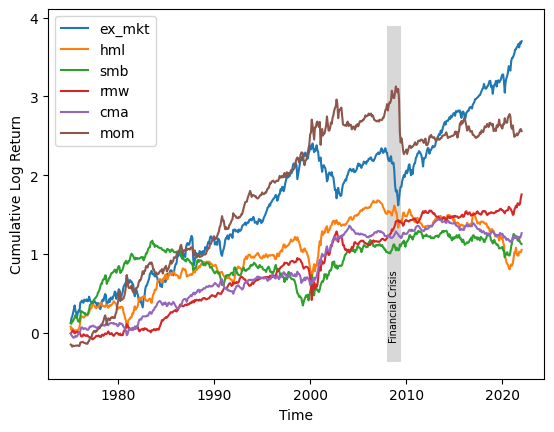
\includegraphics[width=1\textwidth]{plots/cumret_ff.png}
    \caption{This figure shows the cumulative log return of the five factors in the FF five-factor model along with the momentum factor.}
    \label{fig:cumret_ff}
\end{figure}

\newpage


\begin{figure}
  \centering  \captionsetup{justification=raggedright,singlelinecheck=false}
      \caption{Panel A: January 1975 - December 2021 (full sample)}
      \label{fig:betafig}
    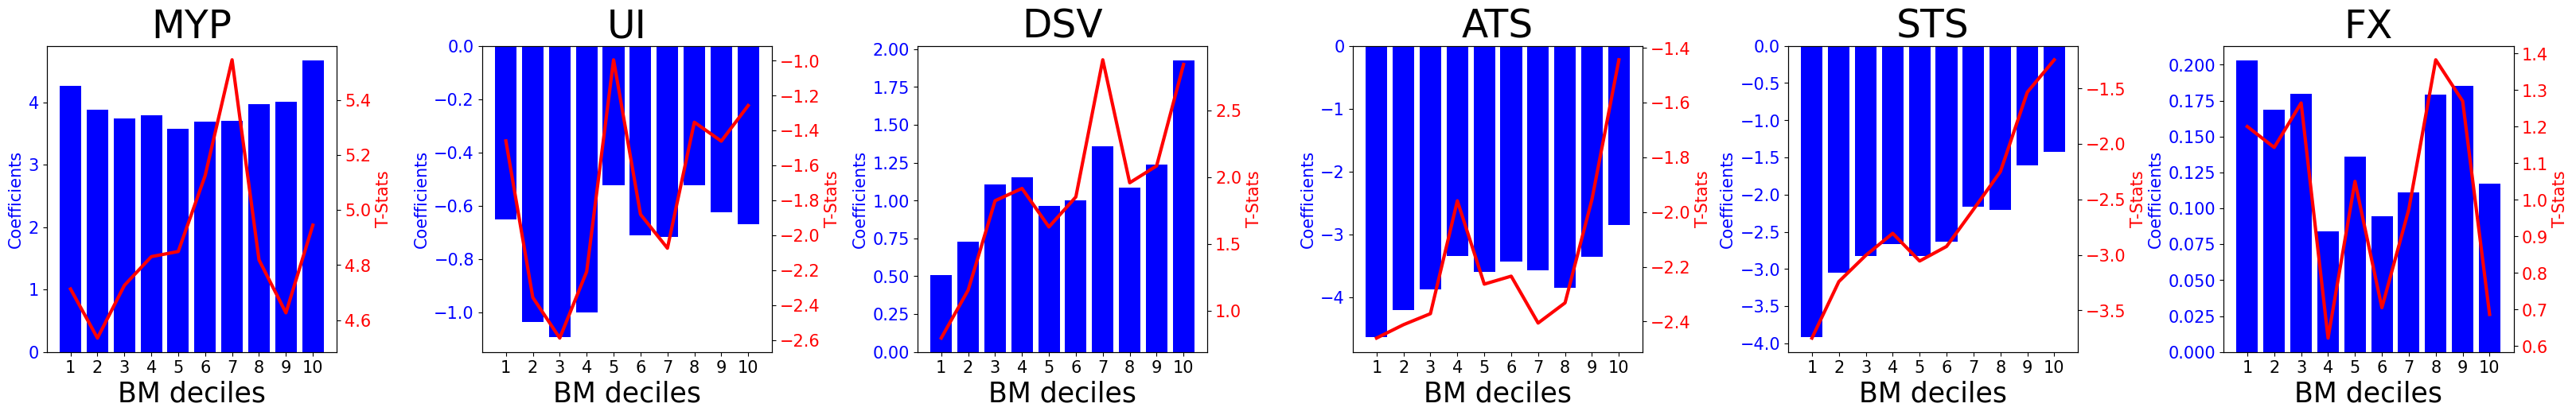
\includegraphics[width=16cm]{plots/betahist1_sample0.png}\\
    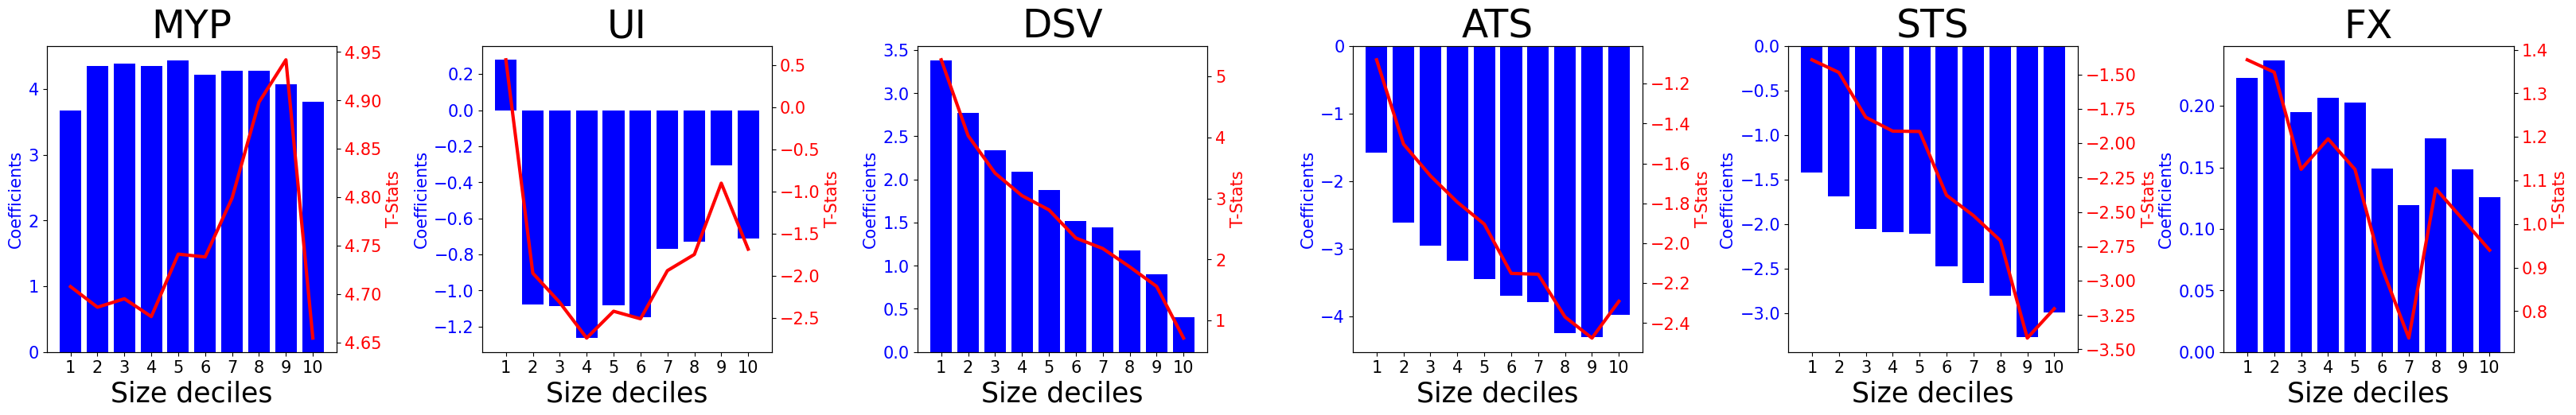
\includegraphics[width=16cm]{plots/betahist2_sample0.png}\\
    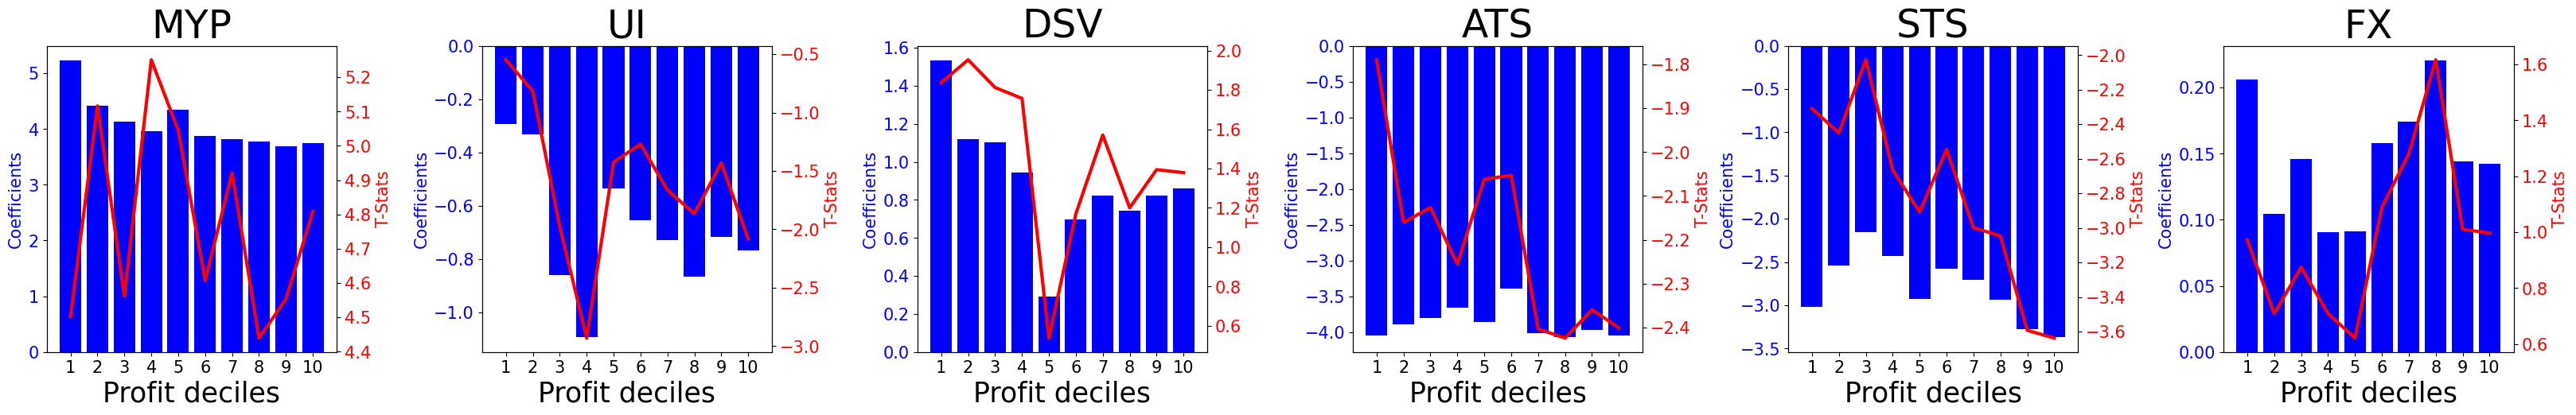
\includegraphics[width=16cm]{plots/betahist3_sample0.png}\\
    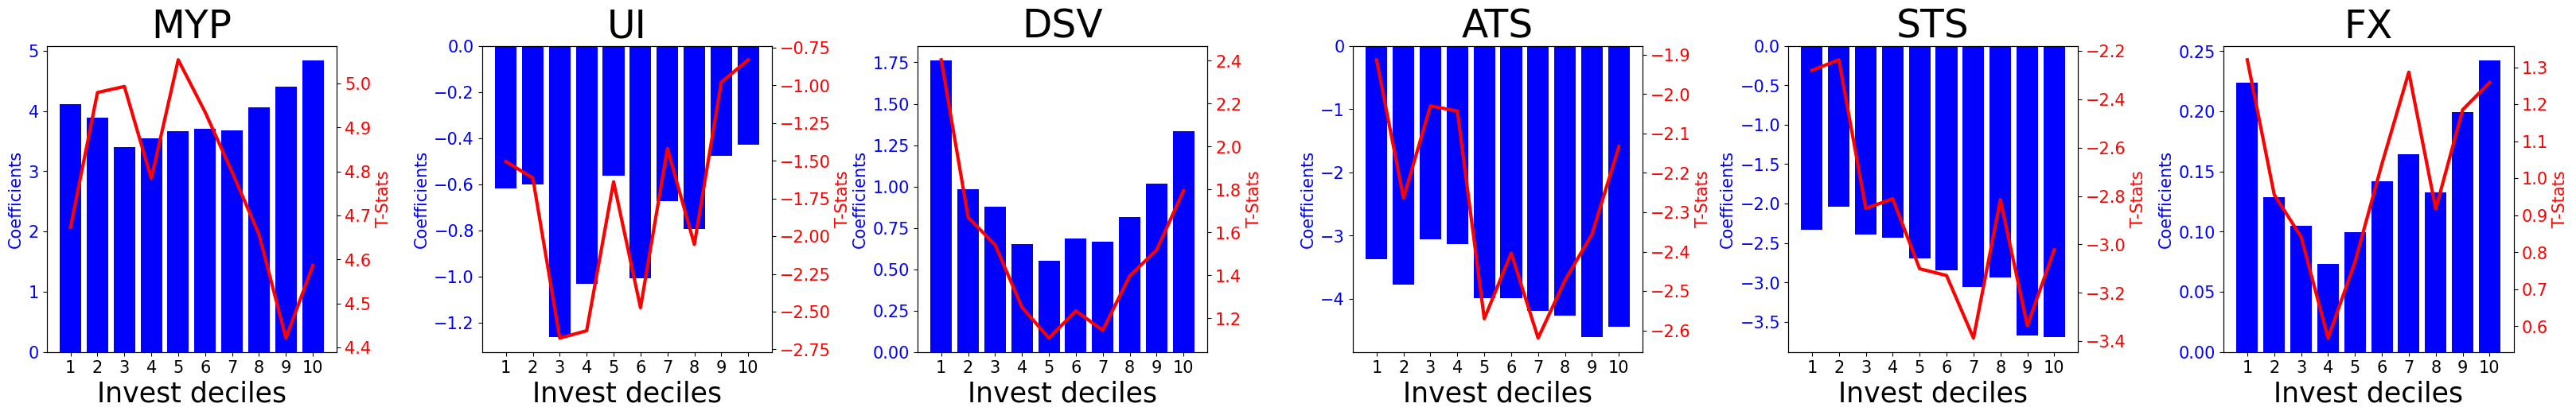
\includegraphics[width=16cm]{plots/betahist4_sample0.png}\\
    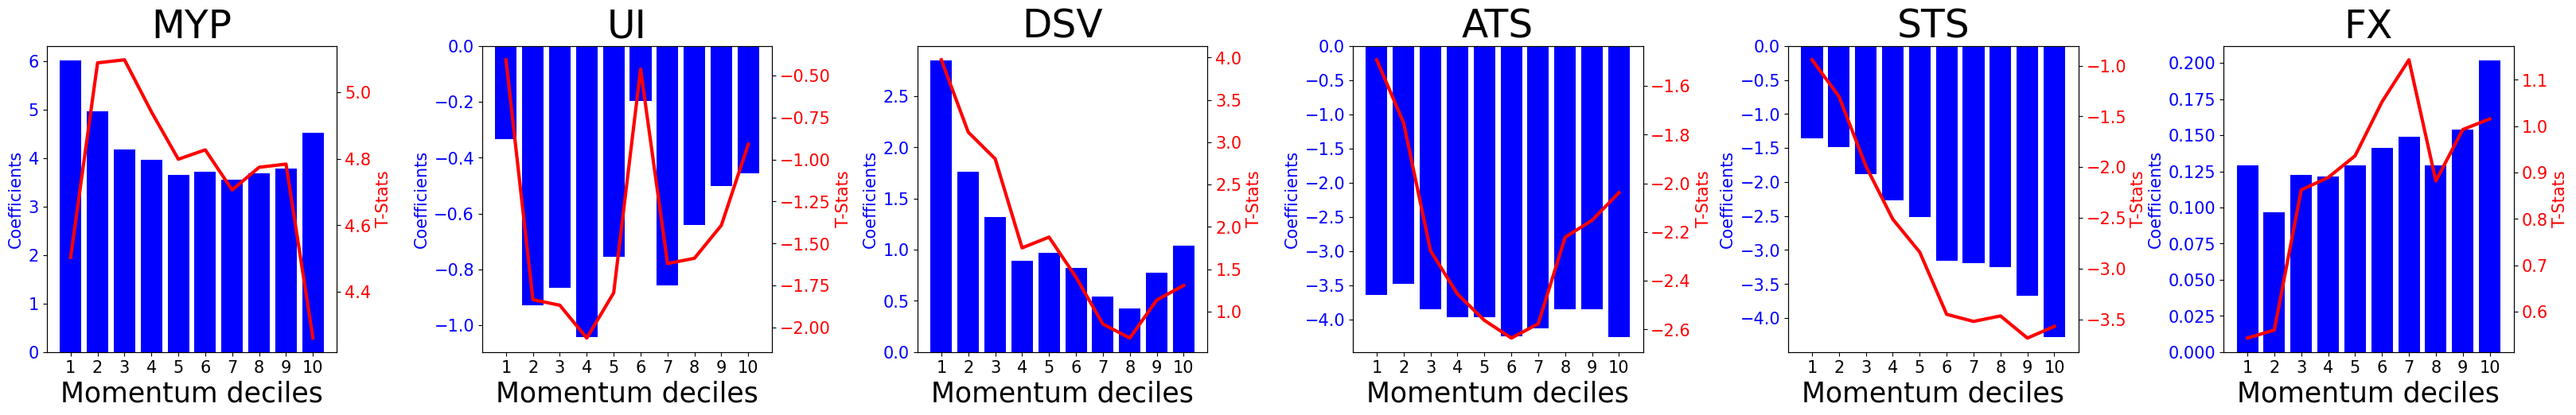
\includegraphics[width=16cm]{plots/betahist5_sample0.png}\\
    % 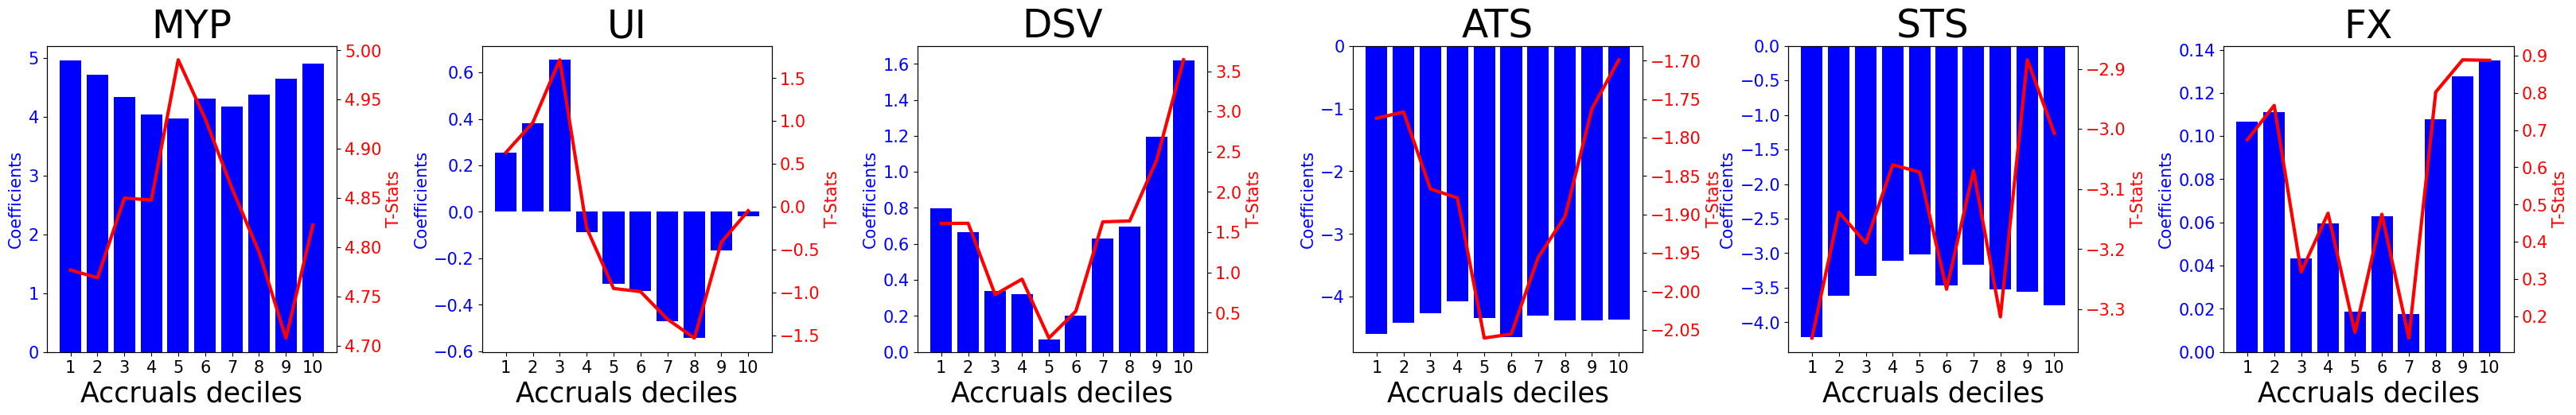
\includegraphics[width=16cm]{plots/betahist6_sample0.png}
\end{figure}
    \clearpage
\begin{figure}\ContinuedFloat
      \centering
    \captionsetup{justification=raggedright,singlelinecheck=false}
      \caption{Panel B: January 1975 - November 2007 (first subsample)}
    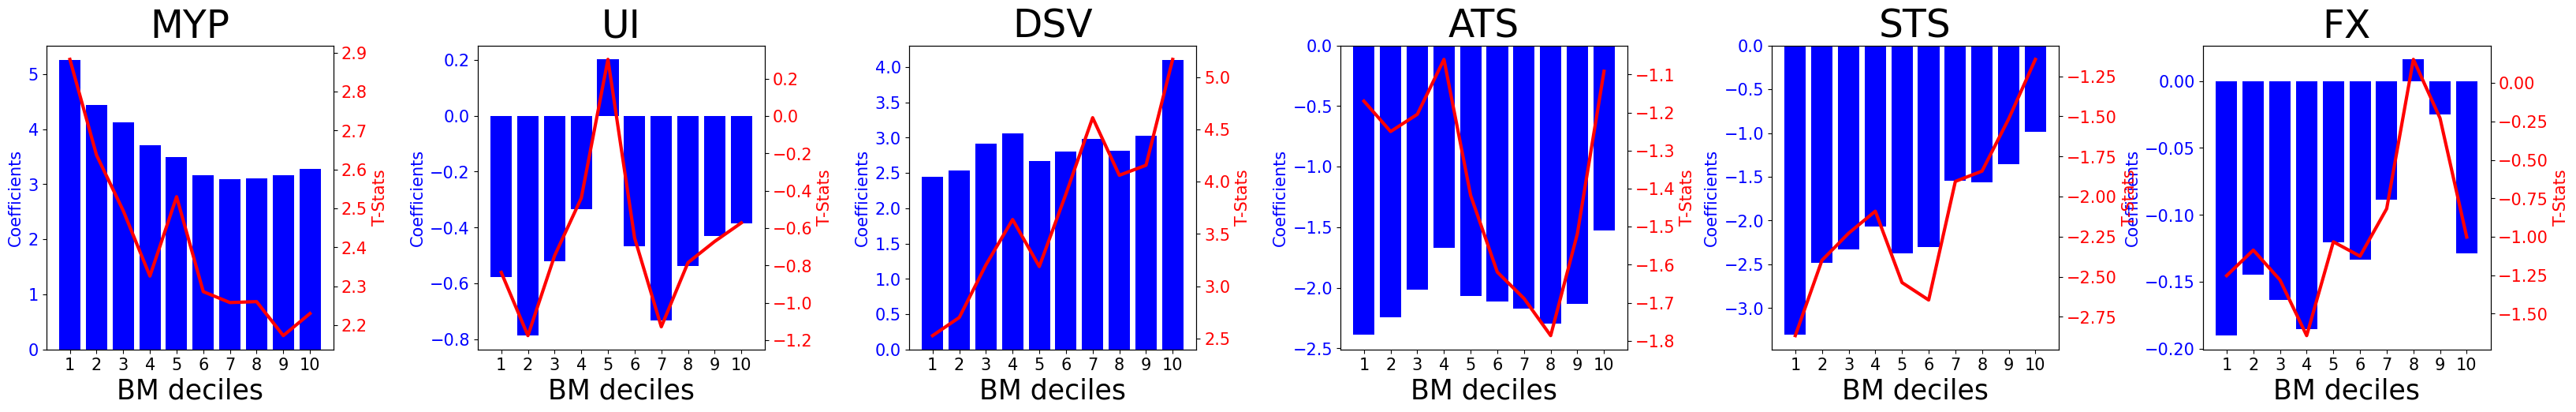
\includegraphics[width=16cm]{plots/betahist1_sample1.png}\\
    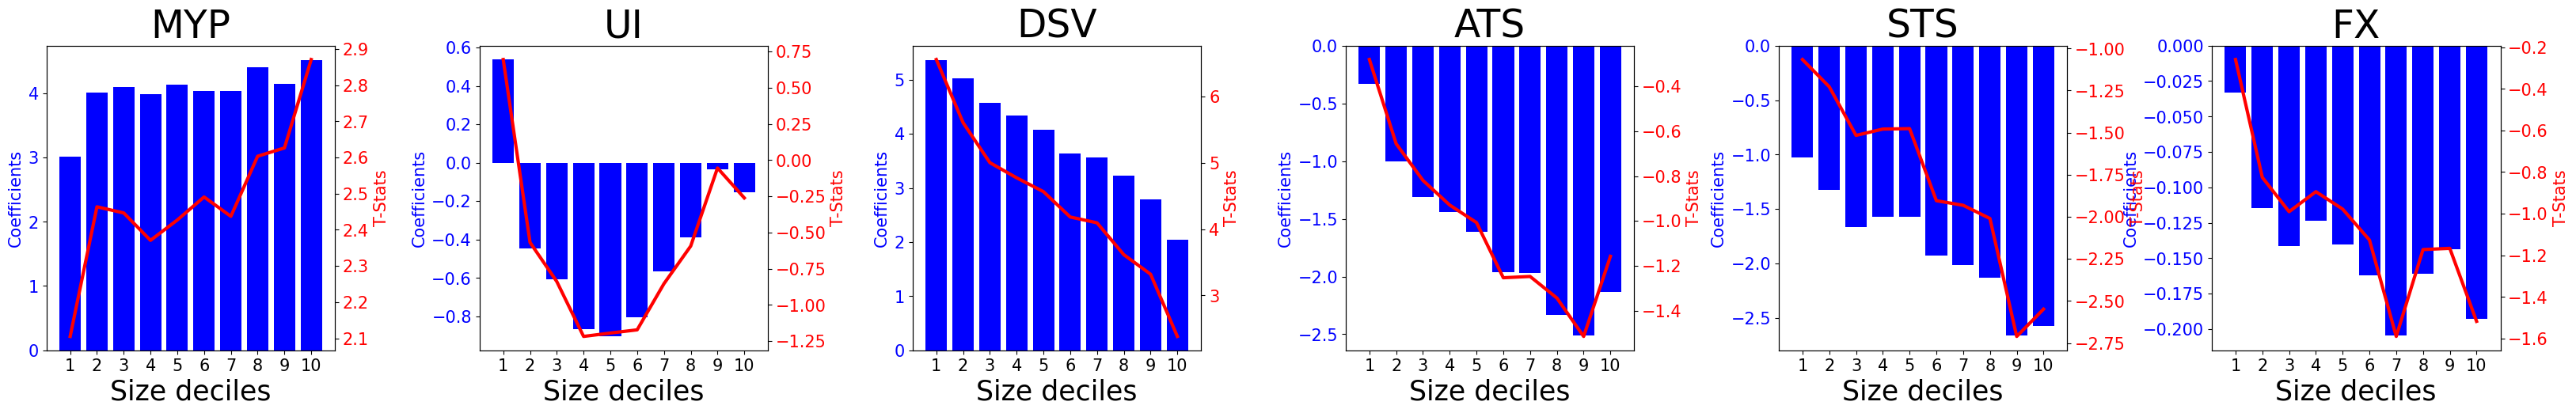
\includegraphics[width=16cm]{plots/betahist2_sample1.png}\\
    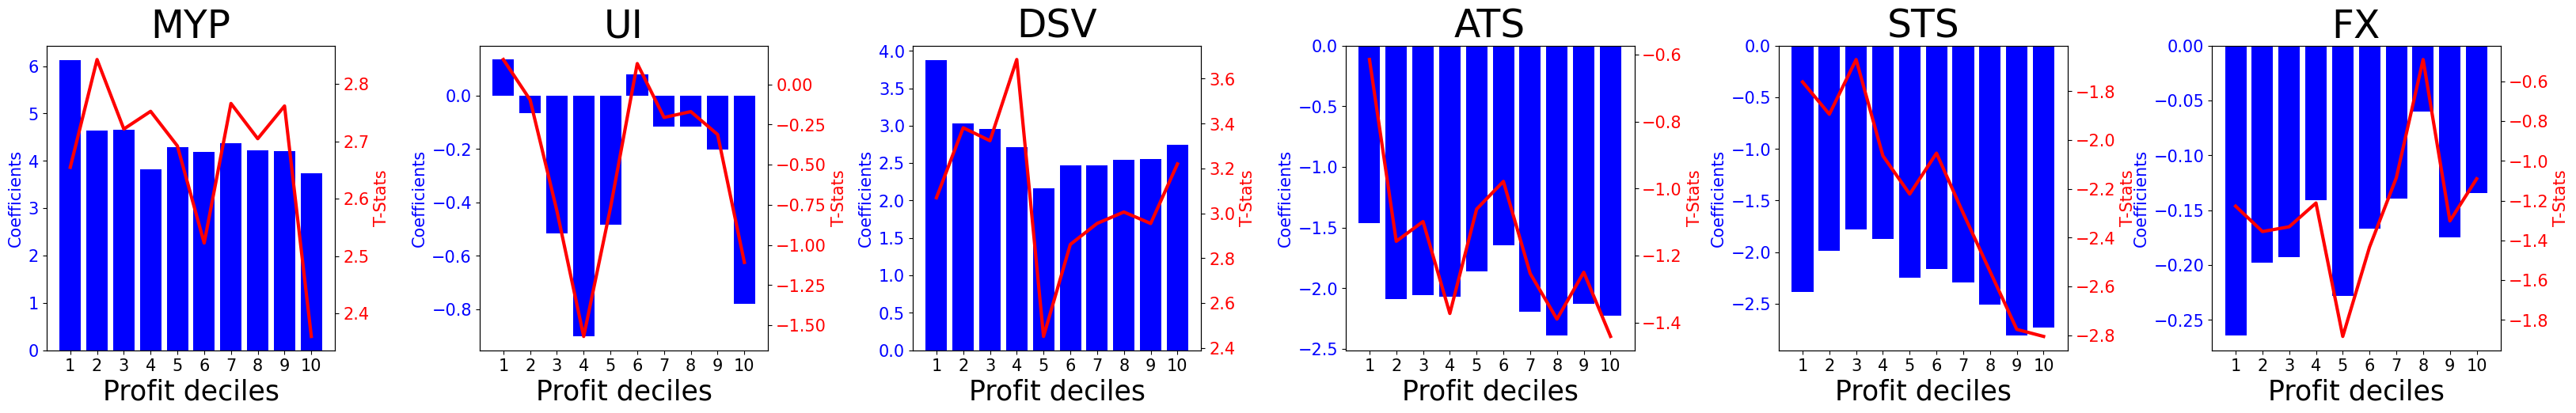
\includegraphics[width=16cm]{plots/betahist3_sample1.png}\\
    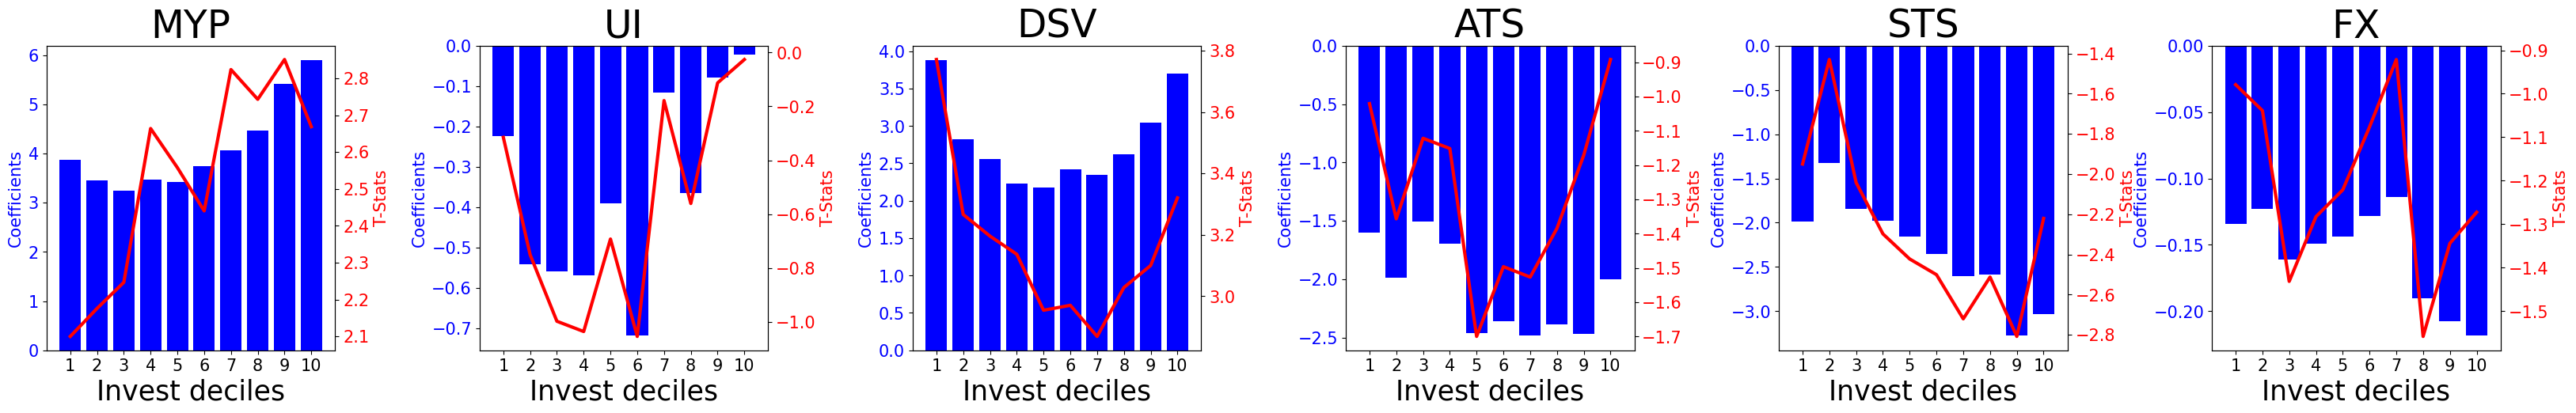
\includegraphics[width=16cm]{plots/betahist4_sample1.png}\\
    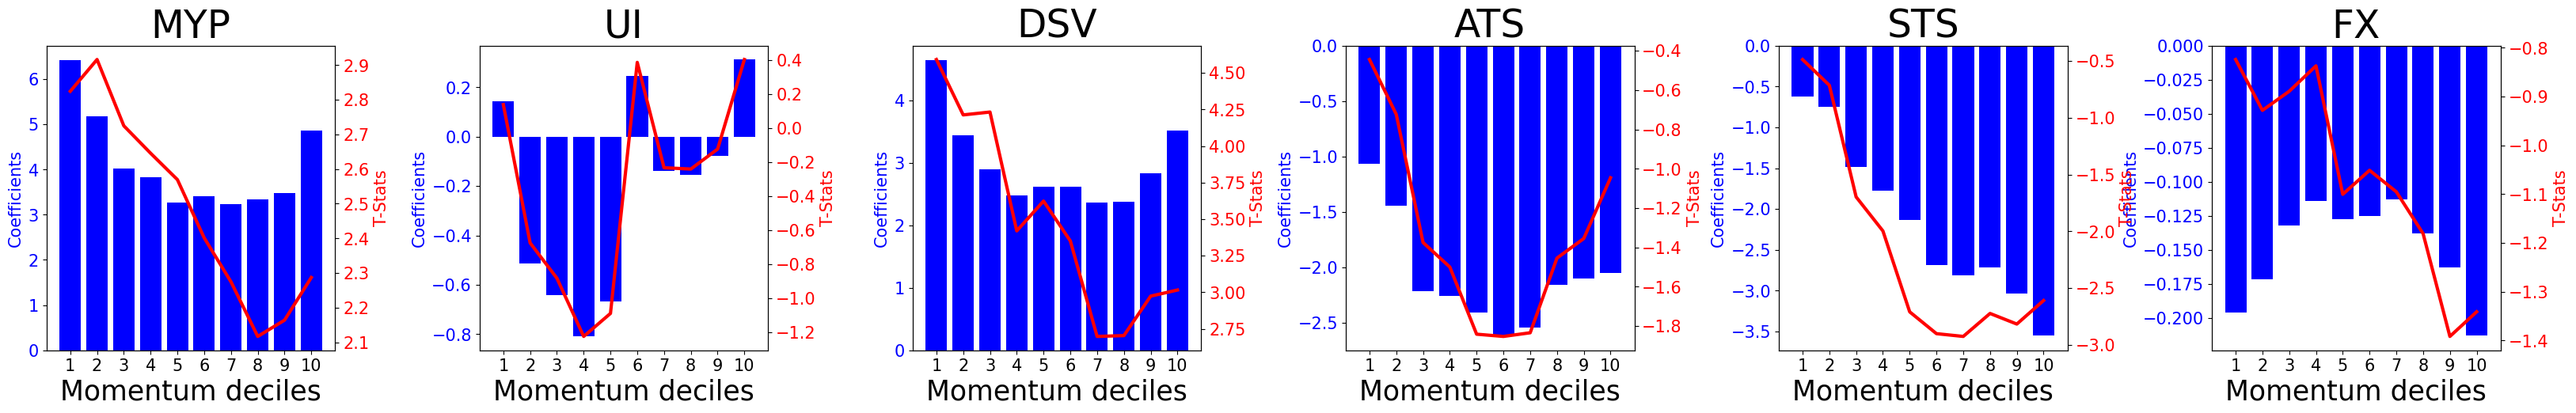
\includegraphics[width=16cm]{plots/betahist5_sample1.png}\\
    % 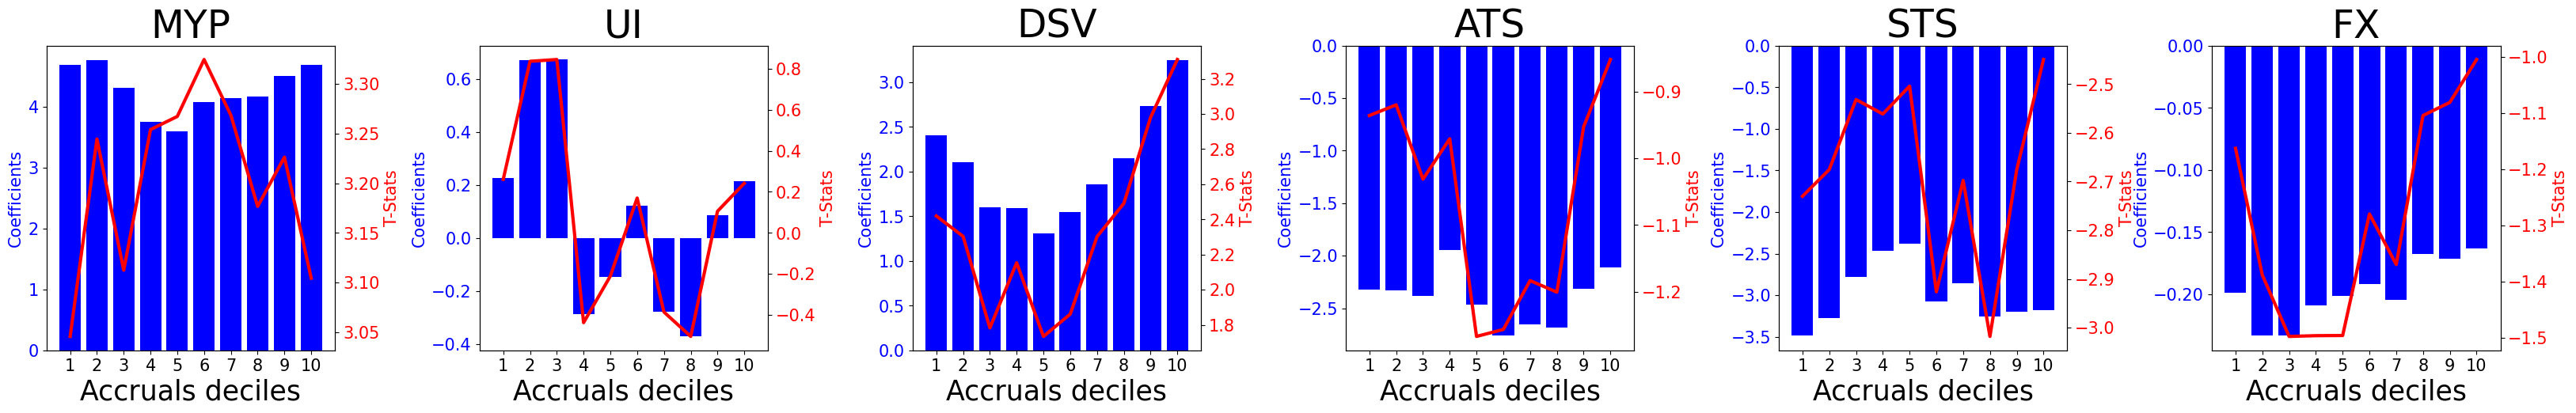
\includegraphics[width=16cm]{plots/betahist6_sample1.png}
\end{figure}
    \clearpage
\begin{figure}\ContinuedFloat
      \centering
    \captionsetup{justification=raggedright,singlelinecheck=false}
      \caption{Panel C: December 2007 - December 2021 (second subsample)}
    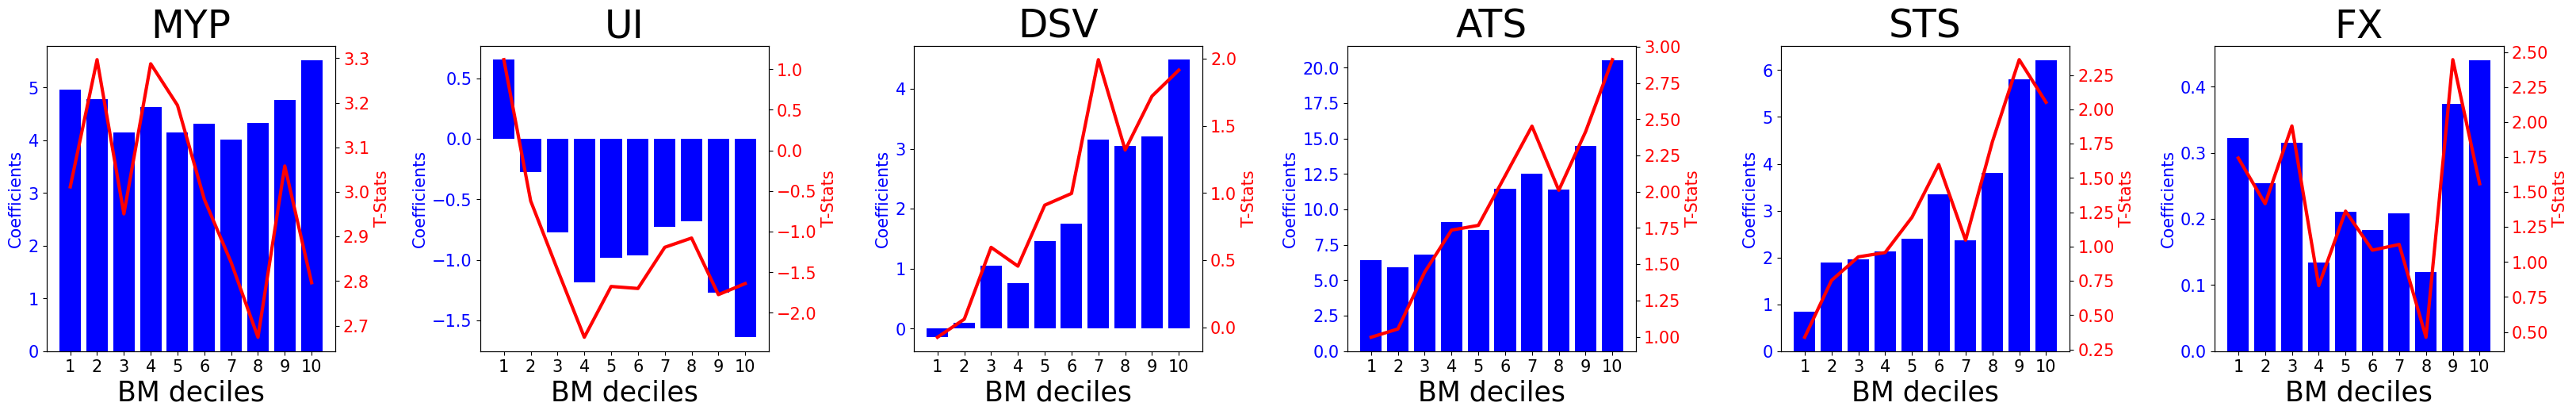
\includegraphics[width=16cm]{plots/betahist1_sample2.png}\\
    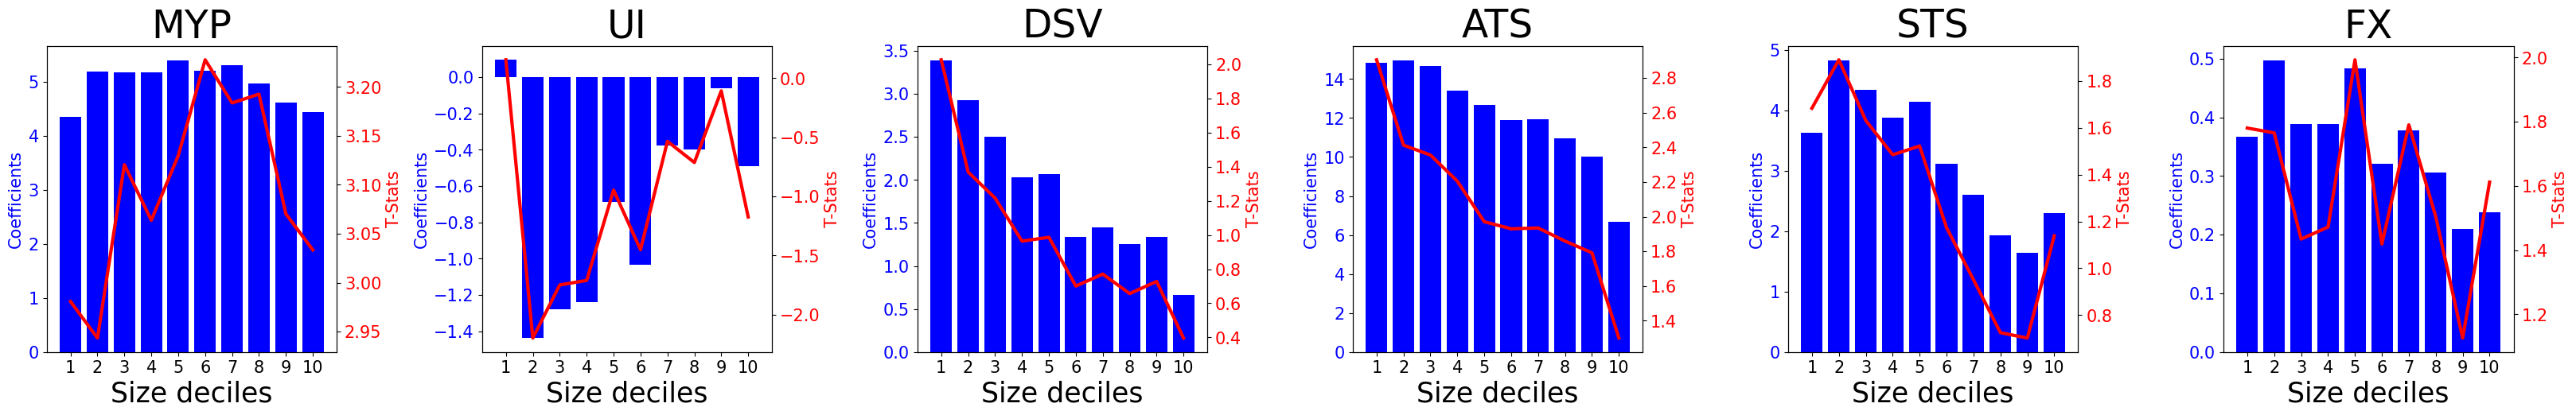
\includegraphics[width=16cm]{plots/betahist2_sample2.png}\\
    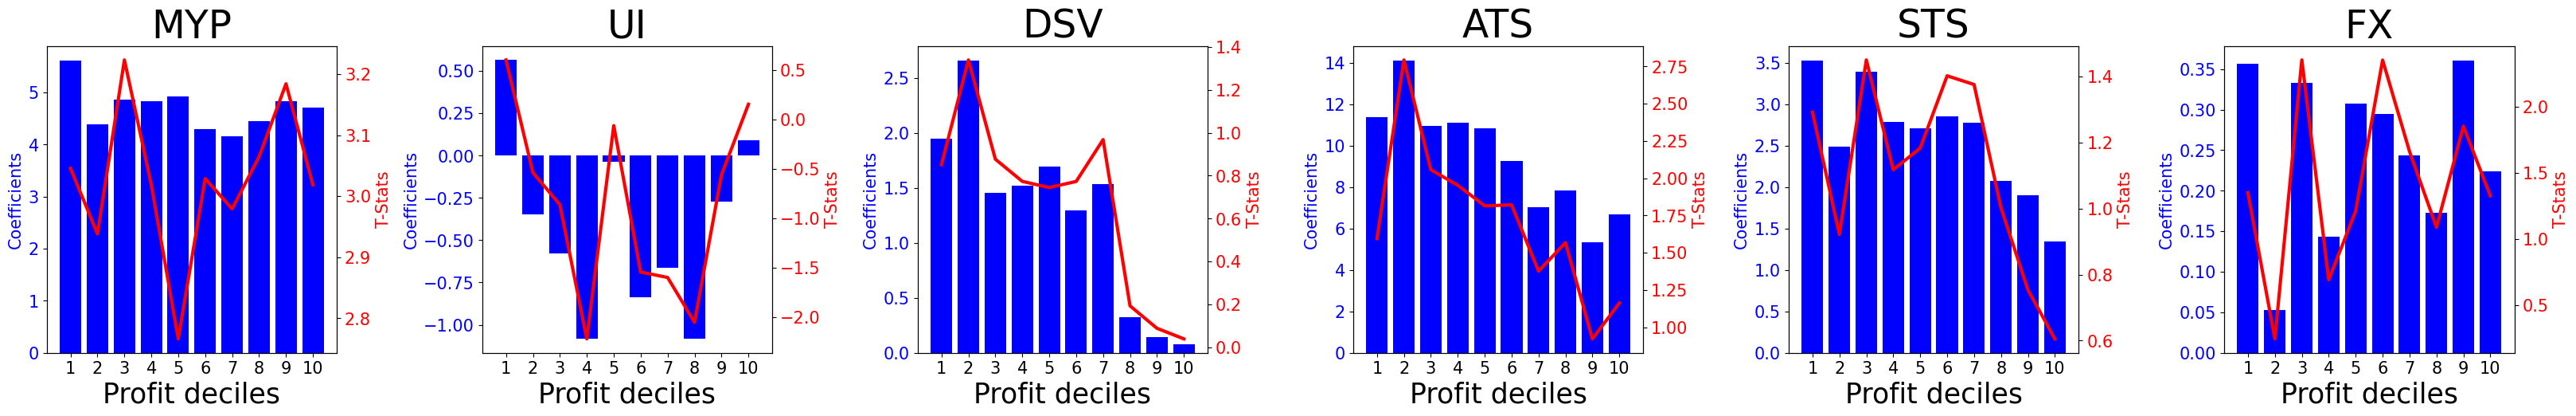
\includegraphics[width=16cm]{plots/betahist3_sample2.png}\\
    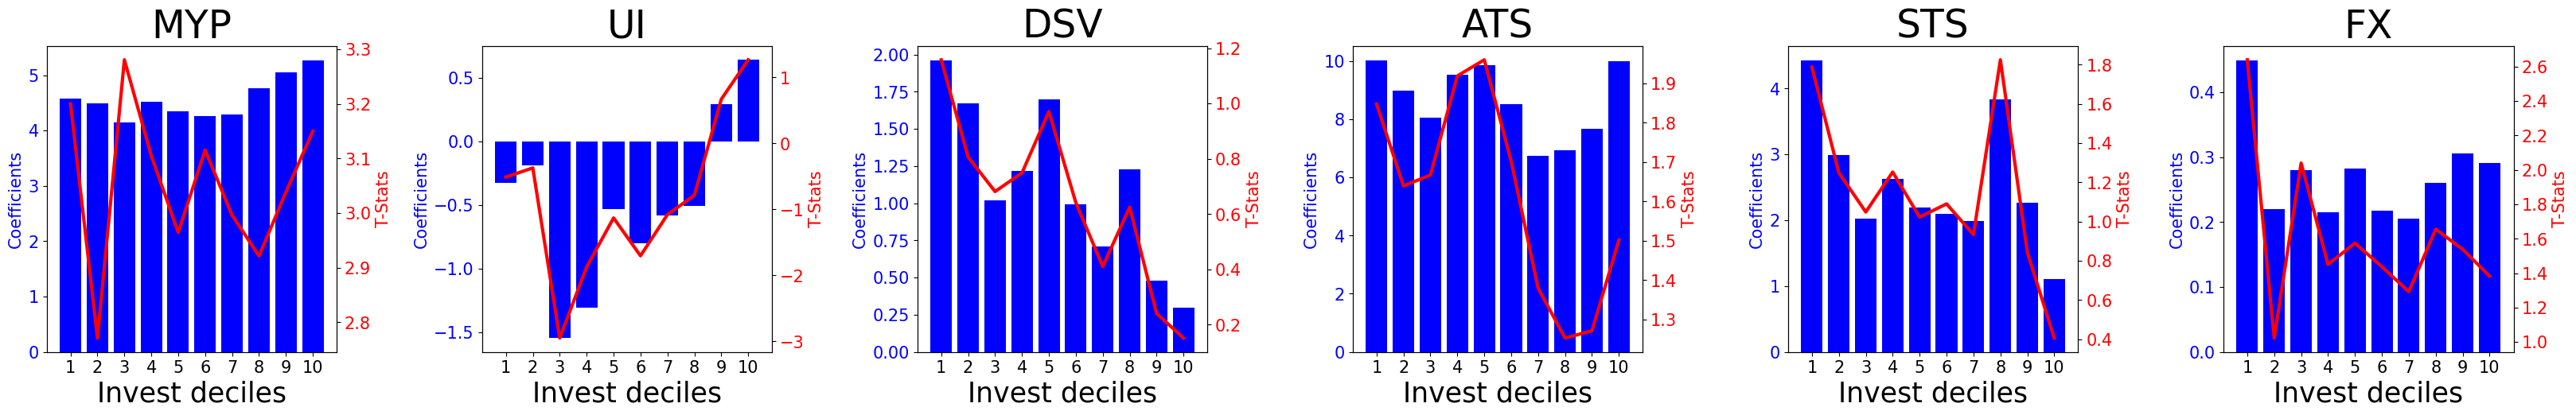
\includegraphics[width=16cm]{plots/betahist4_sample2.png}\\
    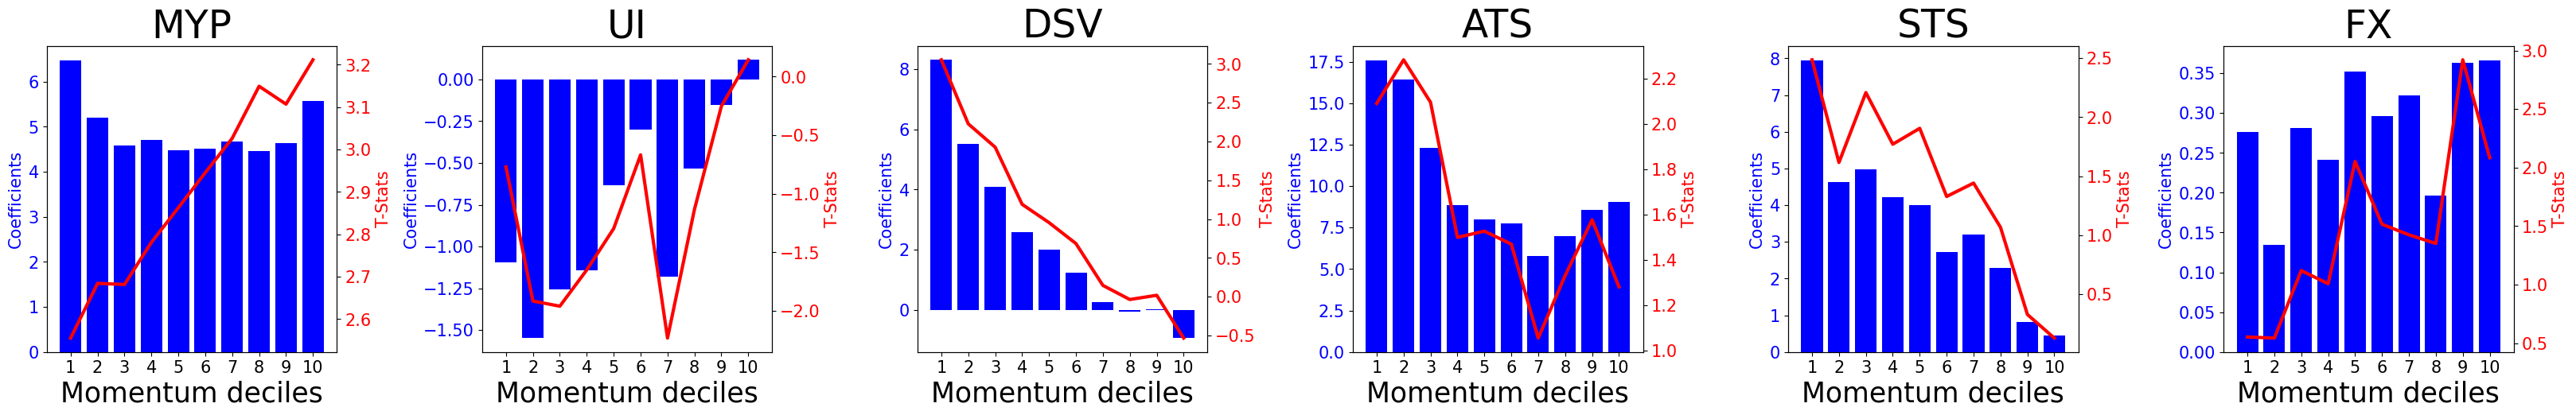
\includegraphics[width=16cm]{plots/betahist5_sample2.png}\\
    % 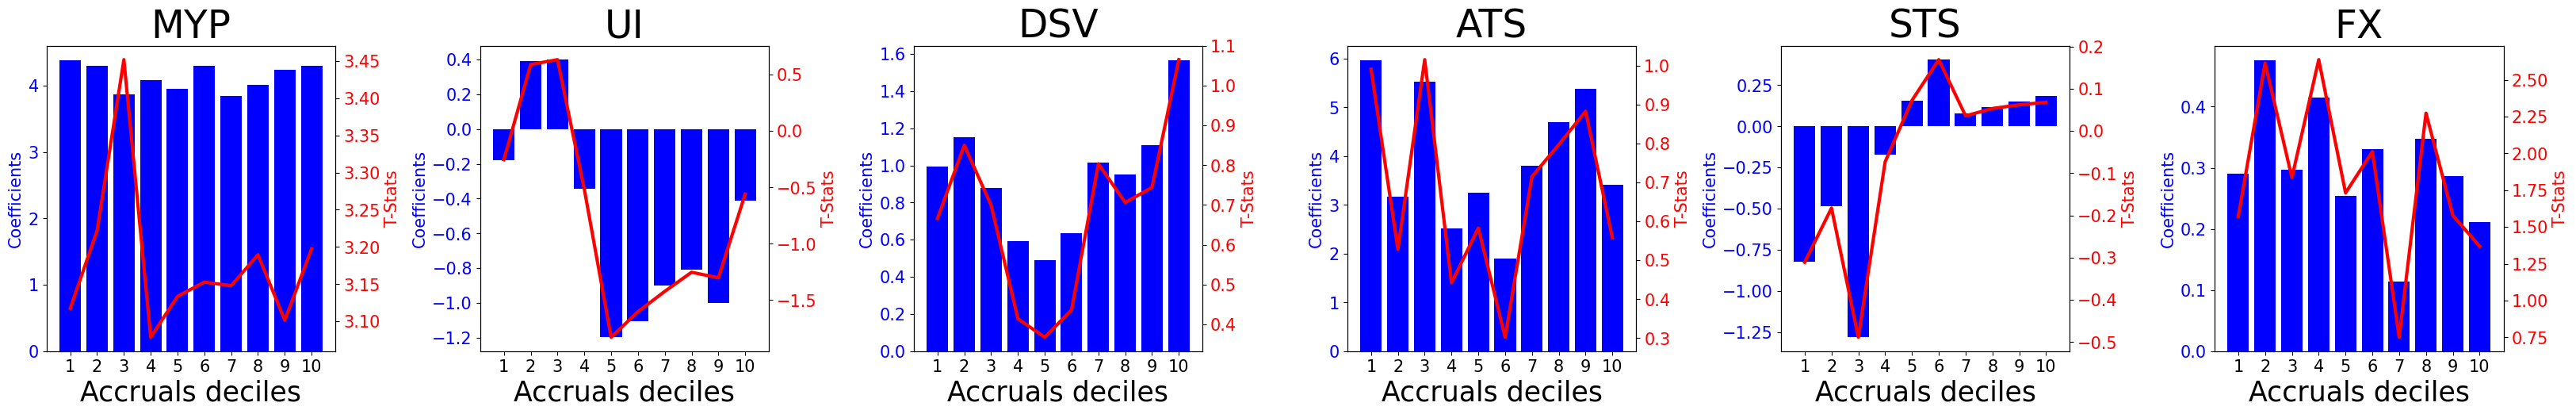
\includegraphics[width=16cm]{plots/betahist6_sample2.png}
\captionsetup{labelformat=empty}
  \caption{This figure shows the macroeconomic risk exposure estimates of the one-way sorted firm characteristic deciles on the macroeconomic fundamentals and their statistics. The macroeconomic fundamentals are changes in industrial production growth expectations (MYP), unexpected inflation (UI), changes in the aggregate survival probability (DSV), changes in the average level and the slope of the term structure of risk-free interest rate yields (ATS and STS, respectively), and changes in the exchange rate between the US dollar and a trade-weighted composite currency (FX). The blue bars are the estimated risk exposures, while the red lines are the t-statistics. The first row shows the outcomes related to the one-way sorted book-to-market deciles, the second those related to the one-way sorted size deciles, the third those related to the one-way sorted momentum deciles, the fourth those related to the one-way sorted operating profitability deciles, the fifth those related to one-way sorted investment deciles, and the sixth those related to one-way sorted accruals deciles. The figures use monthly data (Panel A) from January 1975 to December 2021, (Panel B) from January 1975 to April 2008, and (Panel C) from May 2008 to December 2021.}
\end{figure}

\newpage

\begin{table}
  \begin{threeparttable}
    \caption{Estimation of the mimicking portfolio for industrial production growth}
    \label{tbl:mimick}
    {
\def\sym#1{\ifmmode^{#1}\else\(^{#1}\)\fi}
\begin{tabular}{@{\extracolsep{2pt}}l*{2}{c}@{}}
\hline\hline


 & Ind. productivity growth & Ind. productivity growth \\
\hline
Market portfolio ex. return ($RM_{t-1,t}$) & 0.130 & 0.131 \\
 & (1.547) & (1.515) \\
10-year gov. bond ex. return$_{t-1,t}$ & -0.348\sym{**} & -0.424\sym{**} \\
 & (-2.509) & (-2.262) \\
5-year gov. bond ex. return$_{t-1,t}$ & 0.316\sym{*} & 0.465\sym{**} \\
 & (1.784) & (2.057) \\
Gold ex. returns$_{t-1,t}$ & -0.039 & -0.048\sym{*} \\
 & (-1.452) & (-1.699) \\
Slope dummy mkt portfolio ex. return (87) & -0.079 & -0.081 \\
 & (-0.865) & (-0.968) \\
Slope dummy mkt portfolio ex. return (96-02) & 0.009 & 0.010 \\
 & (0.084) & (0.094) \\
Intercept & 0.025 & 0.026\sym{*} \\
 & (1.606) & (1.703) \\
Risk-free rate of return & -8.787\sym{**} & -9.457\sym{**} \\
 & (-2.031) & (-2.253) \\
10-year minus 3-month gov. bond yield$_{t-1}$ & -0.039 & -0.114 \\
 & (-0.070) & (-0.210) \\
1-year minus 3-month gov. bond yield$_{t-1}$ & 1.814\sym{**} & 1.650\sym{**} \\
 & (2.459) & (2.282) \\
Baa minus Aaa corporate bond yield$_{t-1}$ & -0.352 & -0.298 \\
 & (-0.215) & (-0.185) \\
Dividend yield$_{t-1}$ & 1.656\sym{***} & 1.796\sym{***} \\
 & (2.938) & (3.184) \\
Industrial production growth$_{t-13,t-1}$ & 0.155 & 0.137 \\
 & (1.311) & (1.275) \\
Inflation$_{t-13,t-1}$ & -0.488\sym{**} & -0.510\sym{**} \\
 & (-2.265) & (-2.255) \\
Market portfolio ex. return ($RM_{t-13,t-1}$) & 0.108\sym{***} & 0.101\sym{***} \\
 & (5.418) & (5.589) \\
1-month lagged base asset returns & No & Yes \\

\hline
Obs & 400 & 400 \\
Adj. R\sym{2} & 0.382 & 0.390 \\
F-stat & 10.252 & 8.595 \\
\hline\hline
\end{tabular}
}
    \begin{tablenotes} 
    \footnotesize
    \item This table shows the outcomes from OLS estimations of the log change in industrial production over the next year onto a set of base asset excess returns and lagged control variable realizations. The base assets consist of the market portfolio, 10-year treasury bond return, 5-year treasury bond return, and gold. To allow for time-variation in the market portfolio weight, the regression includes two market portfolio slope dummies for the period from April 1987 to April 1988 (the one year surrounding the October 1987 stock market crash), the period from January 1996 to December 2002 (the Internet bubble period), and the period from December 2007 to May 2009 (the Financial crises). All base asset returns are in excess of the risk-free rate of return, and thus weights do not need to sum up to unity. The regressions control for the expected level of returns by including a set of lagged control variables, containing the risk-free rate, the yield spread between long-term and short-term government bonds, the yield spread between one-year and short-term government bonds, the yield spread between Baa-rated and Aaa-rated corporate bonds and the dividend yield on the S\&P 500. Controls include industrial production growth, inflation, and excess market returns over the last year. Since realized industrial production growth has an overlap with its lagged value of eleven months, the variances have the Newey and West (1987) correction with $l = 11$. The table presents the result for three sample periods: i) from January 1975 to December 2021, ii) from January 1975 to November 2007, and iii) from December 2007 to December 2021.
    \end{tablenotes}
  \end{threeparttable}
\end{table}

\newpage


\begin{table}[htb!]
  \caption{Summary statistics}
  \label{tbl:stats}
  \begin{tabularx}{\linewidth}{l*{9}{Y}}
    \toprule
    \multicolumn{9}{l}{\textbf{Panel A: January 1975 - December 2021 (full sample)}} \\
    \midrule
  
 & N & Mean ($\times 10^3$) & Median ($\times 10^3$) & Std. dev. ($\times 10^3$) & Skew & Kurt & Min. ($\times 10^3$) & Max. ($\times 10^3$) \\
\hline 
 MYP & 564 & 0.869 & 1.391 & 9.991 & -1.185 & 8.385 & 53.421 & -68.452 \\
UI & 564 & -0.037 & -0.109 & 3.166 & -0.765 & 4.101 & 9.222 & -21.147 \\
DSV & 564 & 0.274 & 0.300 & 6.267 & 0.490 & 13.293 & 52.100 & -35.000 \\
ATS & 564 & -0.114 & -0.025 & 3.499 & -1.160 & 14.170 & 18.000 & -28.650 \\
STS & 564 & 0.020 & -0.300 & 3.832 & 0.797 & 5.731 & 21.300 & -15.100 \\
FX & 564 & -0.196 & 0.437 & 18.352 & 0.108 & 2.155 & 92.430 & -65.885 \\


  \end{tabularx}

\begin{tabularx}{\linewidth}{l*{9}{Y}}
    \toprule
    \multicolumn{9}{l}{\textbf{Panel B: January 1975 - November 2007 (first subsample)}} \\
    \midrule
        
 & N & Mean ($\times 10^3$) & Median ($\times 10^3$) & Std. dev. ($\times 10^3$) & Skew & Kurt & Min. ($\times 10^3$) & Max. ($\times 10^3$) \\
\hline 
 MYP & 395 & 0.528 & 0.349 & 5.207 & -0.371 & 2.144 & 16.894 & -21.966 \\
UI & 395 & -0.105 & -0.143 & 2.822 & -0.270 & 1.295 & 9.222 & -11.771 \\
DSV & 395 & 0.353 & 0.323 & 6.764 & 0.597 & 13.195 & 52.100 & -35.000 \\
ATS & 395 & -0.094 & -0.100 & 4.038 & -1.039 & 10.779 & 18.000 & -28.650 \\
STS & 395 & 0.014 & -0.300 & 4.263 & 0.786 & 4.913 & 21.300 & -15.100 \\
FX & 395 & -0.735 & -0.290 & 19.069 & -0.054 & 1.322 & 72.889 & -65.885 \\

 
  \end{tabularx}
  
  \begin{tabularx}{\linewidth}{l*{9}{Y}}
    \toprule
    \multicolumn{9}{l}{\textbf{Panel C: December 2007 - December 2021 (second subsample)}} \\
    \midrule
        
 & N & Mean ($\times 10^3$) & Median ($\times 10^3$) & Std. dev. ($\times 10^3$) & Skew & Kurt & Min. ($\times 10^3$) & Max. ($\times 10^3$) \\
\hline 
 MYP & 169 & 2.378 & 1.822 & 8.847 & -0.632 & 3.390 & 28.310 & -41.739 \\
UI & 169 & 0.119 & -0.031 & 3.857 & -1.238 & 5.260 & 8.008 & -21.147 \\
DSV & 169 & 0.090 & 0.072 & 4.929 & -0.341 & 5.476 & 19.396 & -22.189 \\
ATS & 169 & -0.162 & 0.050 & 1.672 & -1.808 & 7.631 & 3.750 & -8.700 \\
STS & 169 & 0.034 & -0.100 & 2.569 & 0.486 & 1.837 & 10.000 & -7.800 \\
FX & 169 & 1.063 & 1.013 & 16.540 & 0.770 & 5.178 & 92.430 & -47.970 \\

 
        \cr
    \bottomrule 
  \end{tabularx}
  This table provides summary statistics on the analysis variables. The sample periods extend (Panel A) from January 1975 to December 2021, (Panel B) from January 1975 to November 2007, and (Panel C) from December 2007 to December 2021. 
\end{table}

\newpage



\begin{table}[htb!]
  \caption{Correlations}
  \label{tbl:corr}
  \small
  \begin{tabularx}{\linewidth}{l*{13}{Y}}
    \toprule
    \multicolumn{13}{l}{\textbf{Panel A: January 1975 - December 2021 (full sample)}} \\
    \midrule
  
 & RM & HML & SMB & RMW & CMA & MOM & MYP & UI & DSV & ATS & STS & FX \\
RM & 1.00 & -0.19 & 0.26 & -0.24 & -0.36 & -0.15 & 0.83 & -0.04 & 0.55 & -0.06 & -0.01 & -0.17 \\
HML & -0.19 & 1.00 & -0.01 & 0.19 & 0.65 & -0.25 & -0.05 & 0.04 & -0.01 & 0.00 & 0.13 & -0.01 \\
SMB & 0.26 & -0.01 & 1.00 & -0.40 & -0.04 & -0.02 & 0.30 & -0.02 & 0.40 & 0.11 & 0.10 & 0.00 \\
RMW & -0.24 & 0.19 & -0.40 & 1.00 & 0.10 & 0.08 & -0.28 & -0.07 & -0.15 & -0.04 & -0.11 & 0.07 \\
CMA & -0.36 & 0.65 & -0.04 & 0.10 & 1.00 & -0.03 & -0.24 & -0.02 & -0.15 & 0.02 & 0.11 & 0.04 \\
MOM & -0.15 & -0.25 & -0.02 & 0.08 & -0.03 & 1.00 & -0.27 & -0.01 & -0.23 & -0.00 & -0.21 & 0.07 \\
MYP & 0.83 & -0.05 & 0.30 & -0.28 & -0.24 & -0.27 & 1.00 & 0.10 & 0.49 & 0.19 & 0.16 & -0.20 \\
UI & -0.04 & 0.04 & -0.02 & -0.07 & -0.02 & -0.01 & 0.10 & 1.00 & -0.07 & 0.14 & 0.07 & -0.06 \\
DSV & 0.55 & -0.01 & 0.40 & -0.15 & -0.15 & -0.23 & 0.49 & -0.07 & 1.00 & -0.03 & 0.01 & -0.12 \\
ATS & -0.06 & 0.00 & 0.11 & -0.04 & 0.02 & -0.00 & 0.19 & 0.14 & -0.03 & 1.00 & -0.31 & 0.21 \\
STS & -0.01 & 0.13 & 0.10 & -0.11 & 0.11 & -0.21 & 0.16 & 0.07 & 0.01 & -0.31 & 1.00 & -0.09 \\
FX & -0.17 & -0.01 & 0.00 & 0.07 & 0.04 & 0.07 & -0.20 & -0.06 & -0.12 & 0.21 & -0.09 & 1.00 \\


  \end{tabularx}
\begin{tabularx}{\linewidth}{l*{13}{Y}}
    \toprule
    \multicolumn{13}{l}{\textbf{Panel B: January 1975 - November 2007 (first subsample)}} \\
    \midrule
        
 & RM & HML & SMB & RMW & CMA & MOM & MYP & UI & DSV & ATS & STS & FX \\
RM & 1.00 & -0.41 & 0.21 & -0.26 & -0.45 & -0.01 & 0.60 & -0.16 & 0.57 & -0.15 & -0.04 & -0.06 \\
HML & -0.41 & 1.00 & -0.17 & 0.28 & 0.71 & -0.15 & -0.31 & 0.05 & -0.11 & -0.05 & 0.11 & 0.04 \\
SMB & 0.21 & -0.17 & 1.00 & -0.41 & -0.08 & 0.10 & 0.09 & -0.07 & 0.45 & 0.08 & 0.08 & 0.03 \\
RMW & -0.26 & 0.28 & -0.41 & 1.00 & 0.10 & 0.08 & -0.31 & -0.04 & -0.14 & -0.02 & -0.11 & 0.05 \\
CMA & -0.45 & 0.71 & -0.08 & 0.10 & 1.00 & -0.01 & -0.36 & 0.05 & -0.20 & 0.03 & 0.10 & 0.02 \\
MOM & -0.01 & -0.15 & 0.10 & 0.08 & -0.01 & 1.00 & -0.19 & 0.03 & -0.15 & 0.03 & -0.22 & 0.00 \\
MYP & 0.60 & -0.31 & 0.09 & -0.31 & -0.36 & -0.19 & 1.00 & -0.11 & 0.30 & -0.03 & 0.19 & 0.10 \\
UI & -0.16 & 0.05 & -0.07 & -0.04 & 0.05 & 0.03 & -0.11 & 1.00 & -0.13 & 0.13 & 0.03 & 0.01 \\
DSV & 0.57 & -0.11 & 0.45 & -0.14 & -0.20 & -0.15 & 0.30 & -0.13 & 1.00 & -0.02 & 0.04 & -0.03 \\
ATS & -0.15 & -0.05 & 0.08 & -0.02 & 0.03 & 0.03 & -0.03 & 0.13 & -0.02 & 1.00 & -0.37 & 0.25 \\
STS & -0.04 & 0.11 & 0.08 & -0.11 & 0.10 & -0.22 & 0.19 & 0.03 & 0.04 & -0.37 & 1.00 & -0.12 \\
FX & -0.06 & 0.04 & 0.03 & 0.05 & 0.02 & 0.00 & 0.10 & 0.01 & -0.03 & 0.25 & -0.12 & 1.00 \\

 
  \end{tabularx}
% \end{table}
%     \clearpage
% \begin{table}\ContinuedFloat
  \begin{tabularx}{\linewidth}{l*{13}{Y}}
    \toprule
    \multicolumn{13}{l}{\textbf{Panel C: December 2007 - December 2021 (second subsample)}} \\
    \midrule
        
 & RM & HML & SMB & RMW & CMA & MOM & MYP & UI & DSV & ATS & STS & FX \\
RM & 1.00 & 0.27 & 0.40 & -0.21 & -0.11 & -0.40 & 0.89 & 0.17 & 0.53 & 0.41 & 0.07 & -0.47 \\
HML & 0.27 & 1.00 & 0.38 & -0.05 & 0.50 & -0.46 & 0.13 & 0.03 & 0.29 & 0.27 & 0.26 & -0.11 \\
SMB & 0.40 & 0.38 & 1.00 & -0.36 & 0.11 & -0.31 & 0.27 & 0.06 & 0.24 & 0.33 & 0.19 & -0.08 \\
RMW & -0.21 & -0.05 & -0.36 & 1.00 & 0.08 & 0.08 & -0.12 & -0.16 & -0.19 & -0.18 & -0.11 & 0.12 \\
CMA & -0.11 & 0.50 & 0.11 & 0.08 & 1.00 & -0.08 & -0.13 & -0.16 & 0.03 & -0.05 & 0.18 & 0.09 \\
MOM & -0.40 & -0.46 & -0.31 & 0.08 & -0.08 & 1.00 & -0.33 & -0.07 & -0.50 & -0.17 & -0.21 & 0.26 \\
MYP & 0.89 & 0.13 & 0.27 & -0.12 & -0.13 & -0.33 & 1.00 & 0.12 & 0.59 & 0.11 & -0.14 & -0.60 \\
UI & 0.17 & 0.03 & 0.06 & -0.16 & -0.16 & -0.07 & 0.12 & 1.00 & 0.09 & 0.30 & 0.17 & -0.22 \\
DSV & 0.53 & 0.29 & 0.24 & -0.19 & 0.03 & -0.50 & 0.59 & 0.09 & 1.00 & -0.12 & -0.10 & -0.46 \\
ATS & 0.41 & 0.27 & 0.33 & -0.18 & -0.05 & -0.17 & 0.11 & 0.30 & -0.12 & 1.00 & 0.29 & 0.02 \\
STS & 0.07 & 0.26 & 0.19 & -0.11 & 0.18 & -0.21 & -0.14 & 0.17 & -0.10 & 0.29 & 1.00 & 0.03 \\
FX & -0.47 & -0.11 & -0.08 & 0.12 & 0.09 & 0.26 & -0.60 & -0.22 & -0.46 & 0.02 & 0.03 & 1.00 \\

 
        \cr
    \bottomrule 
  \end{tabularx}
  This table shows the correlation matrix between the factors of the FF six-factor model (market excess return, BM, size, profitability, investment, and momentum) and the MF model (industrial production growth expectation, unexpected inflation, changes in aggregate survival probability, change in the average level and the slope of the term structure of the risk-free rate, and changes in the exchange rate). The sample periods extend (Panel A) from January 1975 to December 2021, (Panel B) from January 1975 to April 2008, and (Panel C) from May 2008 to December 2021.
\end{table}

\newpage

% \begin{table}[htb!]
%   \caption{VAR estimation}
%   \label{tbl:var}
%   \scriptsize
%   \begin{tabularx}{\linewidth}{l*{12}{Y}}
%     \toprule
%     \multicolumn{12}{l}{\textbf{Panel A: January 1975 - December 2021 (full sample)}} \\
%     \midrule
%   
& HML& SMB& RMW& CMA& WML& MYP& UI& DSV& ATS& STS& FX\\
\hline
Constant & 0.00 & 0.00\sym{*} & 0.00\sym{**} & 0.00\sym{**} & 0.01\sym{***} & 0.00 & -0.00 & 0.00 & -0.00 & 0.00 & 0.00\\
   & (1.05) & (1.69) & (2.52) & (2.33) & (2.67) & (1.44) & (-1.58) & (0.49) & (-1.27) & (0.16) & (0.39)\\
HML & 0.15\sym{**} & -0.01 & -0.01 & 0.05 & -0.10 & -0.01 & 0.00 & -0.01 & -0.00 & 0.00 & 0.05\\
   & (2.03) & (-0.11) & (-0.20) & (1.02) & (-1.00) & (-0.40) & (0.10) & (-0.58) & (-0.72) & (0.42) & (1.07)\\
SMB & 0.05 & -0.00 & 0.09\sym{**} & 0.01 & 0.05 & 0.01 & 0.01\sym{*} & 0.02\sym{**} & 0.00 & 0.00 & -0.04\\
   & (1.01) & (-0.04) & (2.01) & (0.41) & (0.66) & (0.74) & (1.87) & (2.44) & (0.92) & (0.06) & (-1.29)\\
RMW & -0.03 & -0.00 & 0.19\sym{***} & 0.02 & 0.01 & -0.01 & 0.00 & 0.00 & 0.00 & 0.00 & -0.06\sym{*}\\
   & (-0.41) & (-0.07) & (3.83) & (0.30) & (0.16) & (-0.52) & (0.25) & (0.05) & (0.63) & (0.08) & (-1.71)\\
CMA & 0.08 & -0.03 & 0.03 & 0.06 & 0.08 & -0.00 & 0.01 & -0.01 & -0.00 & 0.01 & -0.10\\
   & (0.73) & (-0.31) & (0.35) & (0.81) & (0.61) & (-0.08) & (0.68) & (-0.41) & (-0.23) & (0.42) & (-1.46)\\
WML & -0.02 & -0.06 & -0.00 & -0.01 & 0.05 & -0.02 & 0.00 & -0.00 & 0.00 & -0.01 & 0.00\\
   & (-0.30) & (-1.48) & (-0.01) & (-0.14) & (0.49) & (-1.54) & (0.54) & (-0.50) & (0.61) & (-1.39) & (0.15)\\
MYP & 0.36\sym{*} & 0.48\sym{***} & -0.11 & 0.09 & -0.46 & 0.18 & 0.08\sym{***} & 0.05 & 0.04 & 0.01 & -0.15\\
   & (1.68) & (2.74) & (-1.05) & (0.75) & (-1.46) & (1.49) & (3.62) & (1.15) & (1.38) & (0.68) & (-1.21)\\
UI & 0.53 & -0.86\sym{**} & 0.74\sym{*} & 0.05 & 0.00 & 0.25 & 0.41\sym{***} & -0.11 & 0.03 & 0.10\sym{**} & -0.17\\
   & (1.28) & (-2.14) & (1.78) & (0.19) & (0.00) & (1.20) & (11.16) & (-1.62) & (0.54) & (2.05) & (-0.80)\\
DSV & -0.34 & -0.21 & 0.21 & 0.01 & 0.45 & -0.05 & -0.04\sym{*} & 0.14 & 0.07\sym{*} & -0.05 & 0.44\sym{**}\\
   & (-1.17) & (-0.67) & (1.26) & (0.08) & (1.07) & (-0.55) & (-1.87) & (1.51) & (1.85) & (-1.09) & (2.53)\\
ATS & -0.99\sym{**} & -0.87\sym{*} & -0.16 & -0.21 & 1.61\sym{**} & -0.40\sym{**} & 0.04 & -0.41\sym{***} & 0.19\sym{***} & -0.22\sym{***} & 0.83\sym{***}\\
   & (-2.02) & (-1.91) & (-0.45) & (-0.76) & (2.22) & (-2.55) & (0.84) & (-3.83) & (2.64) & (-2.64) & (2.80)\\
STS & -0.68\sym{*} & -0.30 & 0.01 & -0.19 & 0.88 & -0.23 & -0.06 & -0.03 & -0.01 & 0.04 & 0.53\sym{**}\\
   & (-1.88) & (-0.80) & (0.03) & (-0.83) & (1.33) & (-1.26) & (-1.26) & (-0.42) & (-0.16) & (0.89) & (2.01)\\
FX & 0.19\sym{***} & 0.04 & 0.06 & 0.05 & -0.09 & -0.02 & -0.02\sym{*} & -0.01 & -0.02 & 0.02\sym{*} & 0.10\sym{***}\\
   & (2.77) & (0.77) & (1.08) & (1.20) & (-0.84) & (-0.88) & (-1.81) & (-0.58) & (-1.48) & (1.88) & (2.74)\\

%   \end{tabularx}
% \begin{tabularx}{\linewidth}{l*{12}{Y}}
%     \toprule
%     \multicolumn{12}{l}{\textbf{Panel B: January 1975 - November 2007 (first subsample)}} \\
%     \midrule
%         
& HML& SMB& RMW& CMA& WML& MYP& UI& DSV& ATS& STS& FX\\
\hline
Constant & 0.00\sym{*} & 0.00\sym{*} & 0.00\sym{*} & 0.00\sym{**} & 0.01\sym{***} & 0.00 & -0.00 & 0.00 & -0.00 & 0.00 & -0.00\\
   & (1.93) & (1.67) & (1.70) & (2.15) & (3.85) & (1.52) & (-1.33) & (0.49) & (-0.73) & (0.22) & (-0.17)\\
HML & 0.14 & -0.01 & 0.00 & 0.04 & -0.22\sym{*} & -0.00 & -0.00 & -0.00 & -0.00 & -0.01 & 0.02\\
   & (1.25) & (-0.11) & (0.05) & (0.48) & (-1.67) & (-0.10) & (-0.32) & (-0.06) & (-0.10) & (-0.91) & (0.47)\\
SMB & 0.11\sym{*} & 0.05 & 0.14\sym{**} & 0.05 & 0.08 & 0.00 & 0.01\sym{*} & 0.03\sym{**} & 0.01 & -0.00 & -0.03\\
   & (1.65) & (0.81) & (2.48) & (1.20) & (0.93) & (0.19) & (1.76) & (2.06) & (0.96) & (-0.18) & (-0.77)\\
RMW & 0.02 & 0.05 & 0.22\sym{***} & 0.07 & 0.00 & -0.03\sym{*} & -0.00 & 0.01 & 0.00 & 0.01 & -0.04\\
   & (0.29) & (0.72) & (3.24) & (0.99) & (0.03) & (-1.73) & (-0.19) & (0.66) & (0.41) & (0.98) & (-0.89)\\
CMA & 0.09 & -0.05 & 0.05 & 0.15 & 0.18 & -0.03 & 0.01 & -0.02 & -0.01 & 0.02 & -0.06\\
   & (0.64) & (-0.34) & (0.51) & (1.39) & (1.21) & (-1.23) & (0.88) & (-0.68) & (-0.89) & (1.30) & (-0.81)\\
WML & -0.08 & -0.11\sym{**} & -0.04 & -0.05 & -0.05 & -0.01 & 0.01 & -0.01 & 0.00 & -0.01 & -0.02\\
   & (-1.14) & (-2.56) & (-0.73) & (-0.87) & (-0.55) & (-0.46) & (1.60) & (-1.00) & (0.58) & (-1.14) & (-0.65)\\
MYP & 0.75\sym{*} & 0.52 & 0.16 & 0.61\sym{*} & -1.28\sym{**} & -0.08 & 0.05 & 0.12 & 0.01 & 0.03 & 0.03\\
   & (1.90) & (0.86) & (0.59) & (1.91) & (-2.45) & (-0.81) & (1.20) & (1.23) & (0.12) & (0.62) & (0.11)\\
UI & 0.67 & -1.24\sym{**} & 0.99\sym{*} & 0.41 & -0.15 & -0.02 & 0.37\sym{***} & -0.16 & 0.04 & 0.13\sym{*} & -0.11\\
   & (1.13) & (-2.20) & (1.66) & (1.02) & (-0.23) & (-0.21) & (7.64) & (-1.54) & (0.64) & (1.87) & (-0.41)\\
DSV & -0.27 & -0.10 & 0.07 & 0.04 & 0.45 & -0.08 & -0.02 & 0.15 & 0.09 & -0.06 & 0.34\sym{*}\\
   & (-0.84) & (-0.28) & (0.38) & (0.19) & (1.05) & (-1.45) & (-1.05) & (1.49) & (1.49) & (-1.18) & (1.89)\\
ATS & -0.94 & -0.58 & -0.19 & -0.26 & 0.64 & -0.08 & 0.06\sym{*} & -0.36\sym{***} & 0.23\sym{***} & -0.22\sym{**} & 0.71\sym{**}\\
   & (-1.63) & (-1.22) & (-0.48) & (-0.75) & (0.87) & (-0.57) & (1.94) & (-3.42) & (2.75) & (-2.37) & (2.15)\\
STS & -0.90\sym{**} & -0.19 & -0.21 & -0.46 & 0.07 & -0.03 & 0.00 & -0.03 & 0.02 & 0.05 & 0.34\\
   & (-2.13) & (-0.41) & (-0.63) & (-1.60) & (0.17) & (-0.37) & (0.12) & (-0.34) & (0.28) & (1.15) & (1.17)\\
FX & 0.12 & -0.00 & 0.03 & -0.01 & 0.06 & 0.01 & -0.01 & -0.02 & -0.03 & 0.02\sym{*} & 0.14\sym{***}\\
   & (1.64) & (-0.02) & (0.49) & (-0.28) & (0.51) & (0.43) & (-0.90) & (-1.03) & (-1.46) & (1.85) & (3.68)\\
 
%   \end{tabularx}
% \end{table}
%     \clearpage
% \begin{table}\ContinuedFloat
%   \begin{tabularx}{\linewidth}{l*{12}{Y}}
%     \toprule
%     \multicolumn{12}{l}{\textbf{Panel C: December 2007 - December 2021 (second subsample)}} \\
%     \midrule
%         
& HML& SMB& RMW& CMA& WML& MYP& UI& DSV& ATS& STS& FX\\
\hline
Constant & -0.00 & 0.00 & 0.00 & 0.00 & -0.00 & 0.00\sym{**} & 0.00 & 0.00 & -0.00 & 0.00 & 0.00\\
   & (-1.12) & (0.51) & (1.25) & (0.31) & (-0.04) & (2.22) & (0.72) & (0.33) & (-1.01) & (0.30) & (0.90)\\
HML & 0.23\sym{***} & 0.05 & 0.06 & 0.11\sym{**} & -0.00 & -0.07\sym{*} & -0.00 & 0.00 & -0.00 & 0.01\sym{*} & 0.12\sym{**}\\
   & (2.71) & (0.62) & (1.15) & (2.56) & (-0.03) & (-1.67) & (-0.21) & (0.05) & (-0.12) & (1.70) & (2.09)\\
SMB & -0.07 & -0.08 & 0.02 & -0.01 & -0.17 & -0.02 & 0.00 & 0.02 & -0.00 & 0.01 & -0.02\\
   & (-0.78) & (-0.53) & (0.42) & (-0.18) & (-1.39) & (-1.15) & (0.10) & (1.31) & (-1.03) & (1.13) & (-0.43)\\
RMW & -0.09 & -0.20 & 0.22\sym{***} & -0.03 & 0.09 & -0.01 & 0.00 & -0.02 & -0.01 & -0.01 & -0.05\\
   & (-0.87) & (-1.57) & (3.98) & (-0.41) & (0.41) & (-0.43) & (0.20) & (-0.81) & (-1.42) & (-0.70) & (-0.88)\\
CMA & 0.11 & -0.01 & -0.08 & -0.10 & -0.07 & 0.15\sym{**} & -0.01 & 0.02 & -0.00 & -0.03\sym{*} & -0.11\\
   & (0.53) & (-0.10) & (-0.67) & (-0.86) & (-0.25) & (2.25) & (-0.41) & (0.72) & (-0.25) & (-1.76) & (-1.00)\\
WML & 0.05 & 0.01 & 0.08\sym{***} & 0.05\sym{*} & 0.21 & -0.03\sym{**} & -0.00 & 0.00 & -0.00 & 0.00 & 0.08\sym{**}\\
   & (1.57) & (0.19) & (2.63) & (1.80) & (1.22) & (-2.48) & (-0.53) & (0.18) & (-0.92) & (0.32) & (2.23)\\
MYP & 0.63 & 0.30 & 0.22 & 0.11 & 0.22 & -0.13 & 0.04 & -0.04 & 0.02 & -0.02 & 0.05\\
   & (1.25) & (0.77) & (0.84) & (0.51) & (0.34) & (-0.80) & (0.88) & (-0.38) & (0.66) & (-0.41) & (0.25)\\
UI & 0.79 & -0.07 & 0.58 & -0.17 & -0.63 & 0.23 & 0.40\sym{***} & 0.05 & 0.04 & 0.02 & -0.29\\
   & (1.18) & (-0.12) & (1.17) & (-0.65) & (-0.53) & (1.00) & (7.58) & (0.49) & (0.89) & (0.34) & (-0.87)\\
DSV & -0.95 & -0.33 & 0.12 & -0.27 & -0.10 & 0.17 & 0.06 & 0.04 & 0.05 & 0.13\sym{**} & 0.20\\
   & (-1.47) & (-0.63) & (0.31) & (-0.86) & (-0.07) & (0.68) & (0.68) & (0.20) & (1.14) & (2.30) & (0.52)\\
ATS & 0.33 & 0.18 & -1.47\sym{*} & 0.11 & 3.23 & 0.14 & 0.61\sym{***} & -0.39 & 0.12 & -0.09 & -0.68\\
   & (0.22) & (0.16) & (-1.66) & (0.16) & (0.87) & (0.35) & (2.89) & (-1.03) & (1.23) & (-0.89) & (-0.89)\\
STS & -0.23 & -0.61 & 0.54 & 0.01 & 4.46\sym{*} & -0.44 & -0.20 & -0.20 & -0.01 & 0.01 & 1.18\sym{*}\\
   & (-0.20) & (-0.68) & (0.93) & (0.03) & (1.88) & (-1.08) & (-1.56) & (-0.73) & (-0.15) & (0.18) & (1.86)\\
FX & 0.22\sym{*} & -0.01 & 0.16 & 0.12 & -0.27 & -0.03 & -0.06\sym{**} & -0.04\sym{*} & -0.01 & 0.01 & -0.02\\
   & (1.84) & (-0.08) & (1.33) & (1.30) & (-1.12) & (-0.47) & (-2.19) & (-1.76) & (-0.49) & (1.03) & (-0.17)\\
 
%         \cr
%     \bottomrule 
%   \end{tabularx}
%   This table reports the empirical outcomes from estimations of VAR systems on the Fama and French and Carhart benchmark factors, i.e., HML, SMB and WML, and the macroeconomic fundamentals. The macroeconomic fundamentals are the mimicking portfolio on changes in industrial production growth expectations (MYP), unexpected inflation (UI), changes in the survival probability (DSV), changes in the average level of the term structure of risk-free interest rate yields (ATS), changes in the slope of the term structure of risk-free interest rate yields (STS) and changes in the exchange rate between the US dollar and a trade-weighted composite currency (FX). This table uses monthly data (a) from January 1975 to December 2021, and (b) from January 1975 to April 2008, and (c) from May 2008 to December 2021 with a lag size equal to one. Numbers in parentheses are t-statistics. The independent variables are lagged by one period.
% \end{table}


% \begin{table}
%   \centering
% \caption{VAR estimation}
%   \begin{threeparttable}
%     % \caption{VAR estimation}
%     \begin{subtable}[b]{\linewidth}
%       \centering      \captionsetup{justification=raggedright,singlelinecheck=false}
%       \caption{January 1975 - December 2021 (full sample)}
%       
& HML& SMB& RMW& CMA& WML& MYP& UI& DSV& ATS& STS& FX\\
\hline
Constant & 0.00 & 0.00\sym{*} & 0.00\sym{**} & 0.00\sym{**} & 0.01\sym{***} & 0.00 & -0.00 & 0.00 & -0.00 & 0.00 & 0.00\\
   & (1.05) & (1.69) & (2.52) & (2.33) & (2.67) & (1.44) & (-1.58) & (0.49) & (-1.27) & (0.16) & (0.39)\\
HML & 0.15\sym{**} & -0.01 & -0.01 & 0.05 & -0.10 & -0.01 & 0.00 & -0.01 & -0.00 & 0.00 & 0.05\\
   & (2.03) & (-0.11) & (-0.20) & (1.02) & (-1.00) & (-0.40) & (0.10) & (-0.58) & (-0.72) & (0.42) & (1.07)\\
SMB & 0.05 & -0.00 & 0.09\sym{**} & 0.01 & 0.05 & 0.01 & 0.01\sym{*} & 0.02\sym{**} & 0.00 & 0.00 & -0.04\\
   & (1.01) & (-0.04) & (2.01) & (0.41) & (0.66) & (0.74) & (1.87) & (2.44) & (0.92) & (0.06) & (-1.29)\\
RMW & -0.03 & -0.00 & 0.19\sym{***} & 0.02 & 0.01 & -0.01 & 0.00 & 0.00 & 0.00 & 0.00 & -0.06\sym{*}\\
   & (-0.41) & (-0.07) & (3.83) & (0.30) & (0.16) & (-0.52) & (0.25) & (0.05) & (0.63) & (0.08) & (-1.71)\\
CMA & 0.08 & -0.03 & 0.03 & 0.06 & 0.08 & -0.00 & 0.01 & -0.01 & -0.00 & 0.01 & -0.10\\
   & (0.73) & (-0.31) & (0.35) & (0.81) & (0.61) & (-0.08) & (0.68) & (-0.41) & (-0.23) & (0.42) & (-1.46)\\
WML & -0.02 & -0.06 & -0.00 & -0.01 & 0.05 & -0.02 & 0.00 & -0.00 & 0.00 & -0.01 & 0.00\\
   & (-0.30) & (-1.48) & (-0.01) & (-0.14) & (0.49) & (-1.54) & (0.54) & (-0.50) & (0.61) & (-1.39) & (0.15)\\
MYP & 0.36\sym{*} & 0.48\sym{***} & -0.11 & 0.09 & -0.46 & 0.18 & 0.08\sym{***} & 0.05 & 0.04 & 0.01 & -0.15\\
   & (1.68) & (2.74) & (-1.05) & (0.75) & (-1.46) & (1.49) & (3.62) & (1.15) & (1.38) & (0.68) & (-1.21)\\
UI & 0.53 & -0.86\sym{**} & 0.74\sym{*} & 0.05 & 0.00 & 0.25 & 0.41\sym{***} & -0.11 & 0.03 & 0.10\sym{**} & -0.17\\
   & (1.28) & (-2.14) & (1.78) & (0.19) & (0.00) & (1.20) & (11.16) & (-1.62) & (0.54) & (2.05) & (-0.80)\\
DSV & -0.34 & -0.21 & 0.21 & 0.01 & 0.45 & -0.05 & -0.04\sym{*} & 0.14 & 0.07\sym{*} & -0.05 & 0.44\sym{**}\\
   & (-1.17) & (-0.67) & (1.26) & (0.08) & (1.07) & (-0.55) & (-1.87) & (1.51) & (1.85) & (-1.09) & (2.53)\\
ATS & -0.99\sym{**} & -0.87\sym{*} & -0.16 & -0.21 & 1.61\sym{**} & -0.40\sym{**} & 0.04 & -0.41\sym{***} & 0.19\sym{***} & -0.22\sym{***} & 0.83\sym{***}\\
   & (-2.02) & (-1.91) & (-0.45) & (-0.76) & (2.22) & (-2.55) & (0.84) & (-3.83) & (2.64) & (-2.64) & (2.80)\\
STS & -0.68\sym{*} & -0.30 & 0.01 & -0.19 & 0.88 & -0.23 & -0.06 & -0.03 & -0.01 & 0.04 & 0.53\sym{**}\\
   & (-1.88) & (-0.80) & (0.03) & (-0.83) & (1.33) & (-1.26) & (-1.26) & (-0.42) & (-0.16) & (0.89) & (2.01)\\
FX & 0.19\sym{***} & 0.04 & 0.06 & 0.05 & -0.09 & -0.02 & -0.02\sym{*} & -0.01 & -0.02 & 0.02\sym{*} & 0.10\sym{***}\\
   & (2.77) & (0.77) & (1.08) & (1.20) & (-0.84) & (-0.88) & (-1.81) & (-0.58) & (-1.48) & (1.88) & (2.74)\\

%     \end{subtable}
%     \end{threeparttable}
% \end{table}
%     \clearpage
% \begin{table}\ContinuedFloat
%   \centering
%   \begin{threeparttable}
%     \begin{subtable}[b]{\linewidth}
%       \centering
%       \setcounter{subtable}{1}      \captionsetup{justification=raggedright,singlelinecheck=false}
%       \caption{January 1975 - April 2008 (first subsample)}
%       
& HML& SMB& RMW& CMA& WML& MYP& UI& DSV& ATS& STS& FX\\
\hline
Constant & 0.00\sym{*} & 0.00\sym{*} & 0.00\sym{*} & 0.00\sym{**} & 0.01\sym{***} & 0.00 & -0.00 & 0.00 & -0.00 & 0.00 & -0.00\\
   & (1.93) & (1.67) & (1.70) & (2.15) & (3.85) & (1.52) & (-1.33) & (0.49) & (-0.73) & (0.22) & (-0.17)\\
HML & 0.14 & -0.01 & 0.00 & 0.04 & -0.22\sym{*} & -0.00 & -0.00 & -0.00 & -0.00 & -0.01 & 0.02\\
   & (1.25) & (-0.11) & (0.05) & (0.48) & (-1.67) & (-0.10) & (-0.32) & (-0.06) & (-0.10) & (-0.91) & (0.47)\\
SMB & 0.11\sym{*} & 0.05 & 0.14\sym{**} & 0.05 & 0.08 & 0.00 & 0.01\sym{*} & 0.03\sym{**} & 0.01 & -0.00 & -0.03\\
   & (1.65) & (0.81) & (2.48) & (1.20) & (0.93) & (0.19) & (1.76) & (2.06) & (0.96) & (-0.18) & (-0.77)\\
RMW & 0.02 & 0.05 & 0.22\sym{***} & 0.07 & 0.00 & -0.03\sym{*} & -0.00 & 0.01 & 0.00 & 0.01 & -0.04\\
   & (0.29) & (0.72) & (3.24) & (0.99) & (0.03) & (-1.73) & (-0.19) & (0.66) & (0.41) & (0.98) & (-0.89)\\
CMA & 0.09 & -0.05 & 0.05 & 0.15 & 0.18 & -0.03 & 0.01 & -0.02 & -0.01 & 0.02 & -0.06\\
   & (0.64) & (-0.34) & (0.51) & (1.39) & (1.21) & (-1.23) & (0.88) & (-0.68) & (-0.89) & (1.30) & (-0.81)\\
WML & -0.08 & -0.11\sym{**} & -0.04 & -0.05 & -0.05 & -0.01 & 0.01 & -0.01 & 0.00 & -0.01 & -0.02\\
   & (-1.14) & (-2.56) & (-0.73) & (-0.87) & (-0.55) & (-0.46) & (1.60) & (-1.00) & (0.58) & (-1.14) & (-0.65)\\
MYP & 0.75\sym{*} & 0.52 & 0.16 & 0.61\sym{*} & -1.28\sym{**} & -0.08 & 0.05 & 0.12 & 0.01 & 0.03 & 0.03\\
   & (1.90) & (0.86) & (0.59) & (1.91) & (-2.45) & (-0.81) & (1.20) & (1.23) & (0.12) & (0.62) & (0.11)\\
UI & 0.67 & -1.24\sym{**} & 0.99\sym{*} & 0.41 & -0.15 & -0.02 & 0.37\sym{***} & -0.16 & 0.04 & 0.13\sym{*} & -0.11\\
   & (1.13) & (-2.20) & (1.66) & (1.02) & (-0.23) & (-0.21) & (7.64) & (-1.54) & (0.64) & (1.87) & (-0.41)\\
DSV & -0.27 & -0.10 & 0.07 & 0.04 & 0.45 & -0.08 & -0.02 & 0.15 & 0.09 & -0.06 & 0.34\sym{*}\\
   & (-0.84) & (-0.28) & (0.38) & (0.19) & (1.05) & (-1.45) & (-1.05) & (1.49) & (1.49) & (-1.18) & (1.89)\\
ATS & -0.94 & -0.58 & -0.19 & -0.26 & 0.64 & -0.08 & 0.06\sym{*} & -0.36\sym{***} & 0.23\sym{***} & -0.22\sym{**} & 0.71\sym{**}\\
   & (-1.63) & (-1.22) & (-0.48) & (-0.75) & (0.87) & (-0.57) & (1.94) & (-3.42) & (2.75) & (-2.37) & (2.15)\\
STS & -0.90\sym{**} & -0.19 & -0.21 & -0.46 & 0.07 & -0.03 & 0.00 & -0.03 & 0.02 & 0.05 & 0.34\\
   & (-2.13) & (-0.41) & (-0.63) & (-1.60) & (0.17) & (-0.37) & (0.12) & (-0.34) & (0.28) & (1.15) & (1.17)\\
FX & 0.12 & -0.00 & 0.03 & -0.01 & 0.06 & 0.01 & -0.01 & -0.02 & -0.03 & 0.02\sym{*} & 0.14\sym{***}\\
   & (1.64) & (-0.02) & (0.49) & (-0.28) & (0.51) & (0.43) & (-0.90) & (-1.03) & (-1.46) & (1.85) & (3.68)\\

%     \end{subtable}
%       \end{threeparttable}
% \end{table}
%     \clearpage
% \begin{table}\ContinuedFloat
%   \centering
%   \begin{threeparttable}
%     \begin{subtable}[b]{\linewidth}
%       \centering      
%       \setcounter{subtable}{2} % set the subtable counter to 2 for the third subtable
%     % \renewcommand{\thesubtable}{\alph{subtable}} % redefine the subtable label to be (a), (b), (c), etc.
%     \captionsetup{justification=raggedright,singlelinecheck=false}
%     \caption{May 2008 - December 2021 (second subsample)}
%       
& HML& SMB& RMW& CMA& WML& MYP& UI& DSV& ATS& STS& FX\\
\hline
Constant & -0.00 & 0.00 & 0.00 & 0.00 & -0.00 & 0.00\sym{**} & 0.00 & 0.00 & -0.00 & 0.00 & 0.00\\
   & (-1.12) & (0.51) & (1.25) & (0.31) & (-0.04) & (2.22) & (0.72) & (0.33) & (-1.01) & (0.30) & (0.90)\\
HML & 0.23\sym{***} & 0.05 & 0.06 & 0.11\sym{**} & -0.00 & -0.07\sym{*} & -0.00 & 0.00 & -0.00 & 0.01\sym{*} & 0.12\sym{**}\\
   & (2.71) & (0.62) & (1.15) & (2.56) & (-0.03) & (-1.67) & (-0.21) & (0.05) & (-0.12) & (1.70) & (2.09)\\
SMB & -0.07 & -0.08 & 0.02 & -0.01 & -0.17 & -0.02 & 0.00 & 0.02 & -0.00 & 0.01 & -0.02\\
   & (-0.78) & (-0.53) & (0.42) & (-0.18) & (-1.39) & (-1.15) & (0.10) & (1.31) & (-1.03) & (1.13) & (-0.43)\\
RMW & -0.09 & -0.20 & 0.22\sym{***} & -0.03 & 0.09 & -0.01 & 0.00 & -0.02 & -0.01 & -0.01 & -0.05\\
   & (-0.87) & (-1.57) & (3.98) & (-0.41) & (0.41) & (-0.43) & (0.20) & (-0.81) & (-1.42) & (-0.70) & (-0.88)\\
CMA & 0.11 & -0.01 & -0.08 & -0.10 & -0.07 & 0.15\sym{**} & -0.01 & 0.02 & -0.00 & -0.03\sym{*} & -0.11\\
   & (0.53) & (-0.10) & (-0.67) & (-0.86) & (-0.25) & (2.25) & (-0.41) & (0.72) & (-0.25) & (-1.76) & (-1.00)\\
WML & 0.05 & 0.01 & 0.08\sym{***} & 0.05\sym{*} & 0.21 & -0.03\sym{**} & -0.00 & 0.00 & -0.00 & 0.00 & 0.08\sym{**}\\
   & (1.57) & (0.19) & (2.63) & (1.80) & (1.22) & (-2.48) & (-0.53) & (0.18) & (-0.92) & (0.32) & (2.23)\\
MYP & 0.63 & 0.30 & 0.22 & 0.11 & 0.22 & -0.13 & 0.04 & -0.04 & 0.02 & -0.02 & 0.05\\
   & (1.25) & (0.77) & (0.84) & (0.51) & (0.34) & (-0.80) & (0.88) & (-0.38) & (0.66) & (-0.41) & (0.25)\\
UI & 0.79 & -0.07 & 0.58 & -0.17 & -0.63 & 0.23 & 0.40\sym{***} & 0.05 & 0.04 & 0.02 & -0.29\\
   & (1.18) & (-0.12) & (1.17) & (-0.65) & (-0.53) & (1.00) & (7.58) & (0.49) & (0.89) & (0.34) & (-0.87)\\
DSV & -0.95 & -0.33 & 0.12 & -0.27 & -0.10 & 0.17 & 0.06 & 0.04 & 0.05 & 0.13\sym{**} & 0.20\\
   & (-1.47) & (-0.63) & (0.31) & (-0.86) & (-0.07) & (0.68) & (0.68) & (0.20) & (1.14) & (2.30) & (0.52)\\
ATS & 0.33 & 0.18 & -1.47\sym{*} & 0.11 & 3.23 & 0.14 & 0.61\sym{***} & -0.39 & 0.12 & -0.09 & -0.68\\
   & (0.22) & (0.16) & (-1.66) & (0.16) & (0.87) & (0.35) & (2.89) & (-1.03) & (1.23) & (-0.89) & (-0.89)\\
STS & -0.23 & -0.61 & 0.54 & 0.01 & 4.46\sym{*} & -0.44 & -0.20 & -0.20 & -0.01 & 0.01 & 1.18\sym{*}\\
   & (-0.20) & (-0.68) & (0.93) & (0.03) & (1.88) & (-1.08) & (-1.56) & (-0.73) & (-0.15) & (0.18) & (1.86)\\
FX & 0.22\sym{*} & -0.01 & 0.16 & 0.12 & -0.27 & -0.03 & -0.06\sym{**} & -0.04\sym{*} & -0.01 & 0.01 & -0.02\\
   & (1.84) & (-0.08) & (1.33) & (1.30) & (-1.12) & (-0.47) & (-2.19) & (-1.76) & (-0.49) & (1.03) & (-0.17)\\

%       \begin{tablenotes}
%         \small
%         \item This table reports the empirical outcomes from estimations of VAR systems on the Fama and French and Carhart benchmark factors, i.e., HML, SMB and WML, and the macroeconomic fundamentals. The macroeconomic fundamentals are the mimicking portfolio on changes in industrial production growth expectations (MYP), unexpected inflation (UI), changes in the survival probability (DSV), changes in the average level of the term structure of risk-free interest rate yields (ATS), changes in the slope of the term structure of risk-free interest rate yields (STS) and changes in the exchange rate between the US dollar and a trade-weighted composite currency (FX). This table uses monthly data (a) from January 1975 to December 2021, and (b) from January 1975 to April 2008, and (c) from May 2008 to December 2021 with a lag size equal to one. Numbers in parentheses are t-statistics. The independent variables are lagged by one period.
%       \end{tablenotes}
%     \end{subtable}
%   \end{threeparttable}
% \end{table}


\newpage

\begin{table}[htb!]
  \caption{Macroeconomic risk exposures}
  \label{tbl:macroexp}
  \begin{tabularx}{\linewidth}{l*{8}{Y}}
    \toprule
    \multicolumn{8}{l}{\textbf{Panel A: January 1975 - December 2021 (full sample)}} \\
    \midrule
  
& Constant& MYP& UI& DSV& ATS& STS& FX\\
\hline
RM & -0.00 & 3.98\sym{***} & -0.68\sym{*} & 0.88 & -3.91\sym{**} & -2.96\sym{***} & 0.14\\
   & (-0.01) & (4.70) & (-1.67) & (1.50) & (-2.27) & (-3.08) & (0.95)\\
HML & -0.00 & -0.38 & 0.31 & 0.29 & 0.75 & 1.33\sym{***} & -0.05\\
   & (-0.53) & (-1.07) & (0.93) & (0.94) & (1.39) & (3.14) & (-0.66)\\
SMB & -0.00 & 0.26 & -0.27 & 1.77\sym{***} & 1.18\sym{***} & 0.90\sym{**} & 0.07\\
   & (-1.44) & (1.20) & (-1.12) & (6.21) & (2.61) & (2.52) & (1.04)\\
RMW & 0.00 & -0.57\sym{**} & -0.31 & -0.08 & -0.01 & -0.47 & 0.00\\
   & (0.31) & (-2.18) & (-0.92) & (-0.41) & (-0.03) & (-1.51) & (0.08)\\
CMA & -0.00 & -0.59\sym{***} & -0.11 & 0.01 & 0.89\sym{**} & 0.98\sym{***} & -0.05\\
   & (-0.51) & (-2.64) & (-0.50) & (0.04) & (2.49) & (3.30) & (-1.03)\\
WML & 0.00\sym{*} & -0.66 & 0.19 & -1.05\sym{**} & -0.54 & -2.31\sym{***} & 0.03\\
   & (1.88) & (-1.36) & (0.40) & (-2.35) & (-0.77) & (-3.70) & (0.35)\\

   
  \end{tabularx}

\begin{tabularx}{\linewidth}{l*{8}{Y}}
    \toprule
    \multicolumn{8}{l}{\textbf{Panel B: January 1975 - November 2007 (first subsample)}} \\
    \midrule
        
& Constant& MYP& UI& DSV& ATS& STS& FX\\
\hline
RM & -0.00 & 4.40\sym{***} & -0.22 & 2.71\sym{***} & -2.04 & -2.47\sym{**} & -0.20\\
   & (-0.75) & (2.75) & (-0.37) & (3.11) & (-1.16) & (-2.45) & (-1.59)\\
HML & 0.00 & -2.01\sym{***} & 0.07 & 0.03 & -0.11 & 1.15\sym{**} & 0.14\sym{*}\\
   & (0.27) & (-2.59) & (0.14) & (0.08) & (-0.13) & (2.30) & (1.78)\\
SMB & -0.00 & -0.50 & -0.33 & 2.19\sym{***} & 1.02\sym{**} & 0.87\sym{**} & 0.05\\
   & (-1.64) & (-1.20) & (-0.91) & (7.86) & (2.03) & (2.37) & (0.71)\\
RMW & -0.00 & -1.42\sym{*} & -0.61 & -0.15 & -0.36 & -0.43 & 0.10\\
   & (-0.46) & (-1.94) & (-1.10) & (-0.63) & (-0.59) & (-1.28) & (1.26)\\
CMA & -0.00 & -1.50\sym{**} & -0.11 & -0.22 & 0.46 & 0.95\sym{***} & 0.05\\
   & (-0.43) & (-2.48) & (-0.32) & (-1.21) & (0.80) & (2.72) & (0.75)\\
WML & 0.00\sym{**} & -0.96 & 0.27 & -0.57 & -0.59 & -2.20\sym{***} & -0.02\\
   & (2.29) & (-0.91) & (0.44) & (-1.16) & (-0.83) & (-3.19) & (-0.18)\\
 
  \end{tabularx}
  \end{table}
    \clearpage
\begin{table}\ContinuedFloat
  
  \begin{tabularx}{\linewidth}{l*{8}{Y}}
    \toprule
    \multicolumn{8}{l}{\textbf{Panel C: December 2007 - December 2021 (second subsample)}} \\
    \midrule
        
& Constant& MYP& UI& DSV& ATS& STS& FX\\
\hline
RM & -0.00 & 4.64\sym{***} & -0.44 & 1.01 & 8.35 & 2.33 & 0.27\sym{*}\\
   & (-0.35) & (3.07) & (-1.00) & (0.58) & (1.55) & (1.06) & (1.74)\\
HML & -0.00 & -0.41 & -1.02\sym{**} & 2.69\sym{***} & 5.82 & 2.73 & -0.05\\
   & (-0.33) & (-1.16) & (-2.25) & (5.27) & (1.34) & (1.42) & (-0.30)\\
SMB & -0.00 & 0.60\sym{*} & -0.52 & 1.28\sym{***} & 5.03\sym{***} & 1.62\sym{**} & 0.19\\
   & (-0.23) & (1.86) & (-1.26) & (2.64) & (2.66) & (2.13) & (1.24)\\
RMW & 0.00\sym{*} & 0.11 & -0.36 & -0.80\sym{*} & -1.85\sym{*} & -0.53 & 0.05\\
   & (1.73) & (0.31) & (-0.91) & (-1.79) & (-1.93) & (-0.91) & (0.52)\\
CMA & 0.00 & -0.30 & -0.76\sym{***} & 0.62 & -0.07 & 1.29\sym{***} & 0.03\\
   & (0.38) & (-1.00) & (-3.46) & (1.54) & (-0.07) & (2.69) & (0.34)\\
WML & -0.00 & -0.05 & 1.04 & -5.17\sym{***} & -5.34\sym{*} & -4.34\sym{**} & 0.11\\
   & (-0.31) & (-0.10) & (1.53) & (-4.94) & (-1.68) & (-2.04) & (0.46)\\
 
        \cr
    \bottomrule 
  \end{tabularx}
  In this table, we show the outcomes from OLS estimations of characteristic portfolio returns onto macroeconomic fundamental realizations. The table shows the estimates and significance levels from the time-series regressions using the factor RM, HML, SMB, RMW, CMA, and WML as dependent variables. The numbers in square parentheses are t-statistics. In the one-step GMM approach, we stack the moment conditions of the mimicking portfolio onto the moment conditions of the asset pricing model. All estimation procedures correct for heteroscedasticity and autocorrelation by using the Newey and West (1987) correction with $l = 12$. The sample periods extend (Panel A) from January 1975 to December 2021, (Panel B) from January 1975 to November 2007, and (Panel C) from December 2007 to December 2021. 
\end{table}

\end{document}